\chapter{Indexation par termes-clés en domaines de spécialité}
\label{chap:main-domain_specific_keyphrase_annotation}
  \chaptercite{
    La multiplication des bases de données et l'information devenue
    \og{}marché\fg{} (donc rentable) ont entraîné d'autres corps de métier à
    s'intéresser à la pratique de l'indexation. Mais ce sont les bibliothécaires
    et documentalistes qui en ont défini les méthodes, les usages et les outils.
  }{
    \newcite{guinchat1996techniquesdocumentaires}
  }{.75\linewidth}{\justify}

  %-----------------------------------------------------------------------------

  \section{Introduction}
  \label{sec:main:domain_specific_keyphrase_annotation-introduction}
    Dans ce chapitre, nous nous intéressons à l'indexation par
    termes-clés en domaines de spécialité. Dans la littérature, l'indexation
    par termes-clés se divise en deux catégories~: l'extraction de termes-clés,
    qui fournit des termes-clés apparaissant dans le contenu du document, et
    l'assignement de termes-clés, qui fournit des termes-clés appartenant à un
    vocabulaire contrôlé et n'apparaissant pas nécessairement dans le document.
    Alors que dans la littérature, l'indexation par termes-clés est
    principalement réalisée au seul moyen de l'extraction de termes-clés, nous
    montrons que l'assignement de termes-clés joue un rôle important en domaines
    de spécialité.

    Nous commençons par décrire le comportement des indexeurs
    professionnels qui maintiennent les bases des données bibliographiques de
    l'Inist (Institut de l'information scientifique et technique), puis nous en
    proposons une automatisation. Les indexeurs professionnels assignent à
    chaque document des termes-clés du domaine (d'un vocabulaire contrôlé), et
    extraient des termes-clés spécifiques au document (hors du vocabulaire
    contrôlé), voir des concepts nouveaux dans le domaine. Pour reproduire ce comportement, nous étendons nos travaux sur
    TopicRank en intégrant dans le graphe de sujets les entrées du vocabulaire
    du domaine.

    Enfin, nous présentons les premiers résultats d'une campagne d'évaluation
    manuelle de nos travaux en domaines de spécialité. Pour cette campagne,
    nous proposons un protocole et des métriques permettant d'évaluer deux
    aspects~: la pertinence des termes-clés extraits/assignés et la quantité
    d'information importante capturée par les termes-clés.

  %-----------------------------------------------------------------------------

  \section{Indexation manuelle en domaines de spécialité}
  \label{sec:main-domain_specific_keyphrase_annotation-manual_keyphrase_annotation}
    En nous fondant sur les  propos recueillis auprès des indexeurs
    professionnels de l'Inist, qui maintient une partie des bases de données
    bibliographiques de la \textsc{Bsn} (Bibliothèque scientifique numérique),
    nous présentons la méthodologie d'indexation manuelle en domaines de
    spécialité.

    \subsection{Principes généraux}
    \label{subsec:main-domain_specific_keyphrase_annotation-manual_keyphrase_annotation-principles}
      L'indexation manuelle de l'Inist est régie par cinq principes généraux~:
      \begin{enumerate}
        \item{Conformité~: les termes-clés doivent être conformes au contenu du
              document et au langage documentaire utilisé dans son domaine~;}
        \item{Exhaustivité~: les termes-clés doivent représenter tous les
              aspects importants du document, même lorsque ceux-ci sont
              implicites~;}
        \item{Homogénéité~: les termes-clés des documents d'un même domaine
              doivent être cohérents et identiques lorsqu'ils représentent le
              même concept~;}
        \item{Spécificité~: les termes-clés doivent décrire le contenu d'un
              document au niveau le plus spécifique et peuvent
              parfois être accompagnés de termes-clés plus génériques afin de
              restituer le contenu du document dans son domaine~;}
        \item{Impartialité~: les termes-clés ne doivent pas être représentatifs
              d'un jugement apporté par l'indexeur.}
      \end{enumerate}

      Ces principes généraux de l'indexation manuelle par termes-clés remettent
      en cause la séparation entre extraction et assignement de termes-clés dans
      le contexte de l'indexation automatique en domaines de spécialité. En
      effet, une indexation par termes-clés à un niveau professionnel doit
      respecter le langage de spécialité employé dans le domaine des documents
      indexés (tâche d'assignement), mais elle doit aussi être exhaustive et
      donc fournir des termes-clés très spécifiques, voir de nouveaux concepts
      (tâche d'extraction).

    \subsection{Ressources}
    \label{subsec:main-domain_specific_keyphrase_annotation-manual_keyphrase_annotation-resources}
      L'indexation par termes-clés réalisée par les indexeurs professionnels de
      l'Inist s'appuie sur plusieurs ressources. Ces dernières sont
      représentatives d'une expertise de terrain dans chaque domaine de
      spécialité (grille d'indexation), d'une expertise terminologique
      (vocabulaire contrôlé) et d'une expertise documentaire (règles de
      préindexation). Elles assurent des conditions de travail propices
      au respect des cinq principes généraux énoncés précédemment.

      \subsubsection{Grille d'indexation}
      \label{subsubsec:main-domain_specific_keyphrase_annotation-manual_keyphrase_annotation-resources-indexing_guidelines}
        De nos jours, la grille d'indexation est un guide transmis de manière
        informelle aux indexeurs. Elle indique les notions à indexer selon le
        domaine de spécialité et peut se traduire par un formulaire à compléter
        pour chaque document (cf tableau~\ref{fig:indexing_grid}). C'est un
        canevas donné à titre indicatif aux indexeurs. Ces derniers sont les
        seuls juges pour décider si elle est adaptée ou non pour indexer un
        document.
        \begin{table}[h!]
          \centering
          \begin{tabular}{l|l}
            \toprule
            \textbf{Champ} & \textbf{Exemple}\\
            \hline
            Théorie linguistique & concept linguistique\\
            Objet d'étude & français~; conjonction~; expression linguistique~; cause\\
            Niveau de description & interprétation sémantique~; relation syntaxique\\
            \bottomrule
          \end{tabular}
          \caption[
            Exemple de remplissage de la grille d'indexation de linguistique
          ]{
            Exemple de remplissage de la grille d'indexation de linguistique,
            pour la notice de linguistique présentée dans la
            figure~\ref{fig:example_inist} (page~\pageref{fig:example_inist})
            \label{fig:indexing_grid}
          }
        \end{table}

        En définissant les notions à indexer, la grille d'indexation contribue
        fortement à l'homogénéité de l'indexations~: les documents d'un même
        domaine sont en partie indexés d'après les mêmes notions. Elle contribue
        aussi à l'exhaustivité~: même les notions implicites doivent faire
        partie de l'indexation.

      \subsubsection{Vocabulaire contrôlé}
      \label{subsubsec:main-domain_specific_keyphrase_annotation-manual_keyphrase_annotation-resources-controlled_vocabulary}
        Le vocabulaire contrôlé est une liste de termes-clés possibles dans un
        domaine de spécialité donné. Cette liste est plus ou moins structurée en
        fonction des domaines\footnote{Lorsqu'elles sont structurées, les listes
        respectent la spécification des thésaurus utilisés par la méthode \textsc{Kea++} (cf
        section~\ref{sec:main-state_of_the_art-automatic_keyphrase_assignment},
        page~\pageref{sec:main-state_of_the_art-automatic_keyphrase_assignment}).}.
        Les termes-clés sont mis en relations s'il sont associés à un même
        concept (par exemple, \og{}nom composé\fg{} et \og{}substantif
        composé\fg{} en linguistique) ou si l'un est l'hyperonyme de l'autre,
        c'est-à-dire plus  générique (par exemple, \og{}allemand\fg{} par
        rapport à \og{}haut-allemand\fg{} et \og{}bas-allemand\fg{}).
        
        En définissant le langage documentaire à utiliser pour indexer les
        documents du même domaine, le vocabulaire contrôlé contribue à la
        conformité et à l'homogénéité de l'indexation. Il n'assure cependant pas
        l'exhaustivité et doit être mis à jour régulièrement, soit par une
        veille terminologique, soit au fur et à mesure des indexations
        manuelles, pour intégrer les nouveaux concepts.

      \subsubsection{Règles de préindexation}
      \label{subsubsec:main-domain_specific_keyphrase_annotation-manual_keyphrase_annotation-resources-preindexing_rules}
        Les règles de préindexation sont des règles qui définissent les
        termes-clés (du vocabulaire contrôlé ou non) à assigner en fonction soit
        (1) d'une unité textuelle qui occurre dans le document, soit (2) d'un
        terme-clé assigné au document. À l'instar du vocabulaire contrôlé, les
        règles de préindexation nécessitent un gros effort de maintenance manuelle.
        
        Couplées avec le vocabulaire contrôlé, les règles de préindexation
        permettent d'assurer la conformité et l'homogénéité de l'indexation.
        Elles contribuent aussi à l'exhaustivité, en permettant l'assignement
        d'aspects implicites dans le document (1), et à la spécificité, en
        restituant le contenu du document dans son domaine grâce à des
        termes-clés génériques (2).

    \subsection{Méthodologie}
    \label{subsec:main-domain_specific_keyphrase_annotation-manual_keyphrase_annotation-methodology}
      Nous distinguons cinq phases lors de l'indexation manuelle par
      termes-clés~:
      \begin{enumerate}
        \item{Choix des ressources à utiliser (grille d'indexation, vocabulaire
              contrôlé et règles de préindexation)~;}
        \item{Utilisation d'un système automatisé de proposition de termes-clés
              à partir des règles de préindexation~;}
        \item{Assignement de termes-clés respectant le langage documentaire
              (dans le vocabulaire contrôlé)~;}
        \item{Assignement de termes-clés génériques afin de replacer les
              termes-clés trop spécifiques dans leur domaine~;}
        \item{Extraction des termes-clés ne respectant pas le langage
              documentaire mais utiles pour décrire le contenu le plus important
              du document.}
      \end{enumerate}

      L'indexation Inist peut être qualifiée de semi-automatique. En effet, la
      deuxième phase est automatisée et systématiquement validée par l'indexeur,
      de sorte à réduire le temps d'indexation et à minimiser d'éventuels
      oublis. Cette phase montre la prise de conscience, dans les organismes
      gestionnaires de bases de données bibliographiques, que l'indexation est
      une tâche difficile et coûteuse à entreprendre manuellement.

    \subsection{Bilan}
    \label{subsec:main-domain_specific_keyphrase_annotation-manual_keyphrase_annotation-conclusion}
      L'indexation manuelle en domaines de spécialité que nous avons présenté
      suit des principes d'indexation que nous retrouvons soit en extraction,
      soit en assignement. Alors qu'en indexation automatique par termes-clés,
      les méthodes d'extraction sont plus étudiées que les méthodes
      d'assignement, nous avons vu que l'indexation réalisée par des indexeurs
      professionnels donne la priorité à l'assignement, et que l'extraction doit
      uniquement servir à la compléter. Actuellement, aucune méthode n'effectue
      à la fois extraction et assignement de termes-clés.

  %-----------------------------------------------------------------------------

  \section{Indexation automatique en domaines de spécialité}
  \label{sec:main-domain_specific_keyphrase_annotation-supervised_automatic_keyphrase_extraction}
    L'indexation automatique par termes-clés est définie comme la tâche qui
    consiste à extraire des termes-clés du contenu d'un document, ou à en
    assigner à partir d'un vocabulaire contrôlé. Alors que dans la
    littérature, l'indexation automatique par termes-clés est presque toujours réduite à la
    seule extraction de termes-clés, nous avons vu en domaines de spécialité
    que les deux catégories d'indexation (extraction et assignement) jouent
    chacune un rôle qui lui est propre.

    Pour réaliser une indexation automatique par termes-clés, nous proposons la
    méthode TopicCoRank. TopicCoRank est, à notre connaissance la seule méthode
    capable de réaliser conjointement extraction et assignement de termes-clés.

    \subsection{TopicCoRank}
    \label{subsec:main-domain_specific_keyphrase_annotation-supervised_automatic_keyphrase_annotation-topiccorank}
      TopicCoRank est une méthode supervisée à base de graphe qui réalise
      simultanément extraction et assignement de termes-clés. Issue de
      TopicRank, elle en modifie les étapes suivantes~: construction du graphe,
      ordonnancement et sélection des termes-clés. La construction du graphe
      étend le graphe de sujet initial de TopicRank en l'unifiant à un graphe
      des termes-clés de référence du domaine~; l'ordonnancement est désormais
      conjoint pour les sujets du document et les termes-clés du domaine~; la
      sélection des termes-clés ajoute la possibilité de puiser dans le graphe
      du domaine afin de réaliser de l'assignement.

      \subsubsection{Construction du graphe}
      \label{subsubsec:main-domain_specific_keyphrase_annotation-supervised_automatic_keyphrase_extraction-topiccorank-graph_construction}
        Afin de réaliser simultanément extraction et assignement de termes-clés,
        TopicCoRank unifie deux graphes représentant le document (graphe de
        sujets) et les termes-clés de référence de son domaine (graphe du
        domaine). Ce dernier graphe est construit à partir des termes-clés de
        référence de documents d'entraînement. Comme \newcite{chaimongkol2013technicaltermextraction} l'ont
        fait avant nous pour l'extraction de termes techniques, nous faisons
        l'hypothèse que les termes-clés de référence des documents
        d'entraînement constituent la terminologie du domaine et nous les
        utilisons comme substituts au vocabulaire contrôlé. Contrairement aux
        termes-clés candidats sélectionnés dans le document, les termes-clés de
        référence ne sont pas redondants et ne sont donc pas groupés. Cette
        hypothèse est forte lorsque les données d'entraînement sont
        issues d'une indexation établie dans un contexte professionnel. Elle
        l'est moins pour les autres données (cf exemple figure~\ref{fig:exemple_topiccorank}).

        Soit le graphe unifié non orienté $G = (N, A =
        A_{\textnormal{\textit{interne}}} \cup
        A_{\textnormal{\textit{externe}}})$. $N$ dénote indifféremment les
        sujets et les termes-clés du domaine. $A$ regroupe les arêtes
        $A_{\textnormal{\textit{interne}}}$, qui connectent deux sujets ou deux
        termes-clés du domaine, et les arêtes
        $A_{\textnormal{\textit{externe}}}$, qui connectent un sujet à un
        terme-clé de référence (cf. figure~\ref{fig:topiccorank_graph}). Le
        graphe de sujets et le graphe du domaine sont unifiés grâce aux arêtes
        $A_{\textnormal{\textit{externe}}}$.
        %
        En considérant le domaine comme une carte conceptuelle, l'objectif des
        arêtes $A_{\textnormal{\textit{externe}}}$ est de connecter le document
        à son domaine par l'intermédiaire des concepts qu'ils partagent. Une
        arête $A_{\textnormal{\textit{externe}}}$ est donc créée entre un sujet
        et un terme-clé du domaine si ce dernier appartient au sujet,
        c'est-à-dire correspond à l'un de ses termes-clés candidats.
        %
%        Une arête
%        $A_{\textnormal{\textit{externe}}}$ est ajoutée pour connecter un sujet
%        et un terme-clé de référence si, et seulement si, le terme-clé fait
%        partie des termes-clés candidats qui composent le sujet
%        (\TODO{exemple}). En d'autres termes, TopicCoRank considère le domaine
%        comme une carte conceptuelle et connecte le document au domaine par
%        l'intermédiaire des concepts qu'ils partagent.
        \begin{figure}
          \newcommand{\xslant}{0.25}
          \newcommand{\yslant}{0}

          \centering
          \begin{tikzpicture}[transform shape, scale=.75]
            % frame
            \node [draw,
                   rectangle,
                   minimum width=.7\linewidth,
                   minimum height=8em,
                   xslant=\xslant,
                   yslant=\yslant] (domain_graph) {};
            \node [above=of domain_graph,
                   xshift=.36\linewidth,
                   yshift=8em,
                   anchor=south east] (domain_graph_label) {termes-clés du domaine};

            \node [draw,
                   circle,
                   above=of domain_graph,
                   xshift=.3\linewidth,
                 yshift=5em] (domain_node1) {$V_1$};
            \node [draw,
                   circle,
                   above=of domain_graph,
                   xshift=-.3\linewidth,
                   yshift=5em] (domain_node2) {$V_2$};
            \node [draw,
                   circle,
                   above=of domain_graph,
                   yshift=5em] (domain_node3) {$V_3$};
            \node [draw,
                   circle,
                   above=of domain_graph,
                   xshift=.15\linewidth,
                   yshift=.75em] (domain_node4) {$V_4$};
            \node [draw,
                   circle,
                   above=of domain_graph,
                   xshift=-.15\linewidth,
                   yshift=.75em] (domain_node5) {$V_5$};

            \draw (domain_node1) -- (domain_node3);
            \draw (domain_node2) -- (domain_node3);
            \draw (domain_node2) -- (domain_node4);
            \draw (domain_node4) -- (domain_node5);
            \draw (domain_node4) -- (domain_node3);

            % document
            \node [draw,
                   rectangle,
                   minimum width=.7\linewidth,
                   minimum height=8em,
                   xslant=\xslant,
                   yslant=\yslant,
                   above=of domain_graph,
                   xshift=-2em] (document_graph) {};
            \node [below=of document_graph,
                   xshift=-.36\linewidth,
                   yshift=-8em,
                   anchor=north west] (document_graph_label) {sujets du document};

            \node [draw,
                   circle,
                   regular polygon sides=8,
                   below=of document_graph,
                   xshift=.3\linewidth,
                   yshift=-5em] (document_node1) {$V_6$};
            \node [draw,
                   circle,
                   regular polygon sides=8,
                   below=of document_graph,
                   xshift=-.3\linewidth,
                   yshift=-5em] (document_node2) {$V_7$};
            \node [draw,
                   circle,
                   regular polygon sides=8,
                   below=of document_graph,
                 yshift=-5em] (document_node3) {$V_8$};
            \node [draw,
                   circle,
                   regular polygon sides=8,
                   below=of document_graph,
                   xshift=.15\linewidth,
                   yshift=-.75em] (document_node4) {$V_9$};

            \draw (document_node2) -- (document_node3);
            \draw (document_node3) -- (document_node1);
            \draw (document_node1) -- (document_node4);
            \draw (document_node3) -- (document_node4);

            % extra link
            \draw [dashed] (document_node2) -- (domain_node2);
            \draw [dashed] (document_node3) -- (domain_node3);
            \draw [dashed] (document_node4) -- (domain_node1);
            \draw [dashed] (document_node3) -- (domain_node4);

            % legend
            \node [right=of document_graph, xshift=2em, yshift=-9.25em] (legend_title) {\underline{Légende~:}};
            \node [below=of legend_title, xshift=-1em, yshift=2em] (begin_inner) {};
            \node [right=of begin_inner] (end_inner) {: $A_\textnormal{\textit{interne}}$};
            \node [below=of begin_inner, yshift=1.5em] (begin_outer) {};
            \node [right=of begin_outer] (end_outer) {: $A_\textnormal{\textit{externe}}$};

            \draw (legend_title.north  -| end_outer.east) rectangle (end_outer.south -| legend_title.west);

            \draw (begin_inner) -- (end_inner);
            \draw [dashed] (begin_outer) -- (end_outer);
          \end{tikzpicture}
          \caption{Illustration du graphe unifié utilisé par TopicCoRank
                   \label{fig:topiccorank_graph}}
        \end{figure}

        Pour permettre un ordonnancement conjoint des sujets et des termes-clés
        du domaine, le schéma de connexion entre deux sujets et entre deux
        termes-clés du domaine (arêtes $A_\textnormal{\textit{interne}}$) doit
        être homogène. En effet, si les conditions de connexion et si la
        pondération des arêtes ne sont pas équivalentes et du
        même ordre de grandeur, alors l'impact du domaine sur
        le document, et du document sur le domaine, sera marginal. Pour
        obtenir un graphe unifié homogène, TopicCoRank connecte deux sujets ou
        deux termes-clés du domaine $n_i$ et $n_j$ lorsqu'ils apparaissent
        dans le même contexte et pondère leur arête par le nombre de fois que
        cela se produit ($\textnormal{poids}(n_i, n_j)$). Lorsqu'il s'agit des sujets, le contexte est
        une phrase du document~; lorsqu'il s'agit des
        termes-clés du domaine, le contexte est l'ensemble des termes-clés de
        référence d'un document d'entraînement. Les contextes
        étant utilisés pour la création du graphe, le graphe de sujets n'est
        plus complet comme celui de TopicRank. Ici, nous utilisons la phrase comme
        alternative à la fenêtre de cooccurrence.

      \subsubsection{Ordonnancement conjoint des sujets et des termes-clés du domaine}
      \label{subsubsec:main-domain_specific_keyphrase_annotation-supervised_automatic_keyphrase_extraction-topiccorank-co_ranking}
        L'ordonnancement conjoint des sujets et des termes-clés du domaine
        établit leur ordre d'importance vis-à-vis du contenu du document et du
        domaine. Pour cela, un score d'importance est attribué simultanément aux
        sujets et aux termes-clés du domaine.
%
        Nous reprenons le principe de la recommandation de TopicRank et
        l'adaptons au problème d'ordonnancement conjoint. Les premières
        hypothèses de recommandation sont donc les mêmes que celle de
        TopicRank~:
        \begin{itemize}
          \item{un sujet est d'autant plus important s'il est fortement connecté
                à un grand nombre de sujets et si les sujets avec lesquels il
                est fortement connecté sont importants~;}
          \item{un terme-clé du domaine est d'autant plus important s'il est
                fortement connecté à un grand nombre de termes-clés du domaine
                et si les termes-clés du domaine avec lesquels il est connecté
                sont importants.}
        \end{itemize}
        Ces hypothèses de recommandation, que nous qualifions d'internes,
        permettent d'établir l'importance des sujets les uns par rapport aux
        autres et l'importance des termes-clés du domaine les uns par rapport
        aux autres. Cependant, elles ne permettent pas de tirer profit des
        relations entre sujets et termes-clés du domaine. Par ailleurs,
        l'importance des termes-clés du domaine ne  dépend pas du document. Nous
        ajoutons donc deux nouvelles hypothèses de recommandation, que nous
        qualifions d'externes~:
        \begin{itemize}
          \item{un sujet est d'autant plus important s'il est représenté par
                (connecté à) des termes-clés du domaine importants~;}
          \item{un terme-clé du domaine est d'autant plus important vis-à-vis
                du contenu du document s'il véhicule (est connecté à) l'un de
                ses sujets importants.}
        \end{itemize}
        Sujets et termes-clés du domaine sont ainsi évalués d'après leur usage
        dans le document et leur importance dans le domaine. L'ordonnancement
        des uns joue un rôle sur celui des autres et permet ainsi d'effectuer
        conjointement extraction et assignement.

        L'équation~\ref{math:topiccorank} montre le calcul de l'importance d'un
        sujet ou d'un terme-clé du domaine à partir de sa recommandation interne
        $R_{\textnormal{\textit{interne}}}$ et de sa recommandation externe
        $R_{\textnormal{\textit{externe}}}$~:
        \begin{align}
          S(n_i) &= (1 - \lambda)\ R_{\textnormal{\textit{externe}}}(n_i) + \lambda\ R_{\textnormal{\textit{interne}}}(n_i)\label{math:topiccorank}\\
          R_{\textnormal{\textit{interne}}}(n_i) &= \sum_{n_j \in A_{\textnormal{\textit{interne}}}(n_i)}{\frac{\textnormal{poids}(n_j, n_i) \times S(n_j)}{\mathlarger\sum_{n_k \in A_{\textnormal{\textit{interne}}}(n_j)}{{\textnormal{poids}(n_j, n_k)}}}}\label{math:rin}\\
          R_{\textnormal{\textit{externe}}}(n_i) &= \sum_{n_j \in A_{\textnormal{\textit{externe}}}(n_i)}{\frac{S(n_j)}{|A_{\textnormal{\textit{externe}}}(n_j)|}}\label{math:rout}
        \end{align}
        où $A_{\textnormal{\textit{interne}}}(n_i)$ représente l'ensemble de
        tous les n\oe{}uds connectés au n\oe{}ud $n_i$ par une arête
        $A_\textnormal{\textit{interne}}$, où
        $A_{\textnormal{\textit{externe}}}(n_i)$ représente l'ensemble de tous
        les n\oe{}uds connectés au n\oe{}ud $n_i$ par une arête
        $A_\textnormal{\textit{externe}}$ et où le facteur $\lambda$ permet
        désormais de définir la recommandation la plus influente entre
        $R_{\textnormal{\textit{interne}}}$ et
        $R_{\textnormal{\textit{externe}}}$. Par défaut, nous définissons
        $\lambda=0,5$.

      \subsubsection{Sélection des termes-clés}
      \label{subsubsec:main-domain_specific_keyphrase_annotation-supervised_automatic_keyphrase_extraction-topiccorank-keyphrase_selection}
        TopicCoRank utilise l'ordre
        d'importance établit avec le score $S$ des sujets et termes-clés du
        domaine pour déterminer les termes-clés du document. Les $k$ n\oe{}uds
        du graphe unifié ayant obtenu les meilleurs scores sont retenus, qu'ils
        soient des sujets ou des termes-clés du domaine.

        Lorsqu'un terme-clé du domaine doit être assigné, une étape de
        vérification supplémentaire est effectuée pour s'assurer que son
        importance calculée relève aussi bien du domaine que du document. En
        effet, il est possible que le graphe du domaine soit constitué de
        composantes connexes, soit de sous-graphes dont les n\oe{}uds ne sont
        connectés qu'entre eux. Dans ce cas, il se peut qu'un terme-clé du
        domaine d'un sous-graphe ne soit connecté, ni directement, ni
        indirectement (par l'intermédiaire d'un autre n\oe{}ud), à un sujet du
        document. Son importance est donc déterminée uniquement à partir du
        domaine et il n'est donc pas pertinent de l'assigner au document.

        Lorsqu'un n\oe{}ud retenu représente un sujet, c'est la même stratégie
        que celle de Topic\-Rank qui est appliquée. Pour un sujet donné, le
        terme-clé extrait est son terme-clé candidat qui apparaît en premier
        dans le document.

      \subsubsection{Exemple}
      \label{subsubsec:main-domain_specific_keyphrase_annotation-supervised_automatic_keyphrase_extraction-topiccorank-exemple}
        La figure~\ref{fig:exemple_topiccorank} donne un exemple d'extraction
        et d'assignement de
        termes-clés avec TopicCoRank à partir de la notice d'archéologie
        présentée dans la figure~\ref{fig:example_inist} (page~\pageref{fig:example_inist}). Dans cet exemple,
        nous observons une meilleure indexation par termes-clés qu'avec
        TopicRank. Tout d'abord, nous voyons que le graphe du domaine permet
        l'assignement du termes-clés générique \og{}France\fg{}. Ensuite, nous
        voyons que les relations de \og{}diffusion\fg{}, \og{}analyse\fg{} et
        \og{}répartition\fg{} dans le graphe du domaine permettent de mieux les
        ordonner.
        \begin{figure} % archeologie_525-02-11060
  \centering
  \framebox[\linewidth]{
    \parbox{.99\linewidth}{\footnotesize
      \textbf{Étude préliminaire de la céramique non tournée micacée du bas
      Languedoc occidental : typologie, chronologie et aire de diffusion}\\

      L'étude présente une variété de céramique non tournée dont la
      typologie et l'analyse des décors permettent de l'identifier
      facilement. La nature de l'argile enrichie de mica donne un aspect
      pailleté à la pâte sur laquelle le décor effectué selon la méthode du
      brunissoir apparaît en traits brillant sur fond mat. Cette première
      approche se fonde sur deux séries issues de fouilles anciennes menées
      sur les oppidums du Cayla à Mailhac (Aude) et de Mourrel-Ferrat à
      Olonzac (Hérault). La carte de répartition fait état d'échanges ou de
      commerce à l'échelon macrorégional rarement mis en évidence pour de la
      céramique non tournée. S'il est difficile de statuer sur l'origine des
      décors, il semble que la production s'insère dans une ambiance
      celtisante. La chronologie de cette production se situe dans le
      deuxième âge du Fer. La fourchette proposée entre la fin du
      IV$^\text{e}$ et la fin du II$^\text{e}$ s. av. J.-C. reste encore à
      préciser.\\

      \textbf{Termes-clés de référence~:} distribution~; mourrel-ferrat~;
      olonzac~; le cayla~; mailhac~; micassé~; céramique non-tournée~; celtes~;
      production~; echange~; commerce~; cartographie~; habitat~; oppidum~; site
      fortifié~; fouille ancienne~; identification~; décor~; analyse~;
      répartition~; diffusion~; chronologie~; typologie~; céramique~; etude du
      matériel~; hérault~; aude~; france~; europe~; la tène~; age du fer.
    }
  }~\\

  \vspace{1.5em}

  \newcommand{\xslant}{0.25}
  \newcommand{\yslant}{0}
  \centering
  \begin{tikzpicture}[transform shape, scale=.75]
    % domain %%%%%%%%%%%%%%%%%%%%%%%%%%%%%%%%%%%%%%%%%%%%%%%%%%%%%%%%%%%%%%%%%%%
    \node [draw,
           rectangle,
           minimum width=1.15\linewidth,
           minimum height=.26\textheight,
           xslant=\xslant,
           yslant=\yslant] (domain_graph) {};
    \node [above=of domain_graph,
           xshift=.585\linewidth,
           yshift=.26\textheight,
           anchor=south east] (domain_graph_label) {termes-clés du domaine (sous-partie)};

    % nodes
    \node [above=of domain_graph,%draw,
           xshift=-1.9em,
           yshift=.23\textheight] (france) {france};
    \node [above=of domain_graph,%draw,
           xshift=-7.3em,
           yshift=.18\textheight] (typologie) {typologie};
    \node [above=of domain_graph,%draw,
           xshift=4.3em,
           yshift=.18\textheight] (chronologie) {chronologie};
    \node [above=of domain_graph,%draw,
           xshift=-20em,
           yshift=.14\textheight] (ceramique) {céramique};
    \node [above=of domain_graph,%draw,
           xshift=16.25em,
           yshift=.14\textheight] (production) {production};
    \node [above=of domain_graph,%draw,
           xshift=2.2em,
           yshift=.059\textheight] (analyse) {analyse};
    \node [above=of domain_graph,%draw,
           xshift=-5.2em,
           yshift=.055\textheight] (decor) {décor};
    \node [above=of domain_graph,%draw,
           xshift=-14em,
           yshift=.005\textheight] (repartition) {répartition};
    \node [above=of domain_graph,%draw,
           xshift=10.5em,
           yshift=.009\textheight] (diffusion) {diffusion};

    % france
    \draw (france) -- (typologie);
    \draw (france) -- (chronologie);
    \draw (france) -- (production);
    \draw (france) -- (diffusion);
    \draw (france) -- (decor);
    \draw (france) -- (analyse);
    \draw (france) -- (repartition);
    \draw (france) -- (ceramique);
    % typologie
    \draw (typologie) -- (chronologie);
    \draw (typologie) -- (production);
    \draw (typologie) -- (diffusion);
    \draw (typologie) -- (decor);
    \draw (typologie) -- (analyse);
    \draw (typologie) -- (repartition);
    \draw (typologie) -- (ceramique);
    % chronologie
    \draw (chronologie) -- (production);
    \draw (chronologie) -- (diffusion);
    \draw (chronologie) -- (decor);
    \draw (chronologie) -- (analyse);
    \draw (chronologie) -- (repartition);
    \draw (chronologie) -- (ceramique);
    % production
    \draw (production) -- (diffusion);
    \draw (production) -- (decor);
    \draw (production) -- (analyse);
    \draw (production) -- (ceramique);
    % diffusion
    \draw (diffusion) -- (decor);
    \draw (diffusion) -- (analyse);
    \draw (diffusion) -- (ceramique);
    % decor
    \draw (decor) -- (analyse);
    \draw (decor) -- (ceramique);
    % analyse
    \draw (analyse) -- (ceramique);

    % document %%%%%%%%%%%%%%%%%%%%%%%%%%%%%%%%%%%%%%%%%%%%%%%%%%%%%%%%%%%%%%%%%
    \node [draw,
          rectangle,
          minimum width=1.15\linewidth,
          minimum height=.26\textheight,
          xslant=\xslant,
          yslant=\yslant,
          above=of domain_graph,
          xshift=-3.9em] (document_graph) {};
    \node [below=of document_graph,
           xshift=-.585\linewidth,
           yshift=-.26\textheight,
           anchor=north west] (document_graph_label) {sujets du document (sous-partie)};

    \node [minimum width=2.5em,
           below=of document_graph,%draw,
           xshift=-3.4em,
           yshift=-.025\textheight] (typologie_c) {[typologie]};
    \node [minimum width=2.5em,
           below=of document_graph,%draw,
           xshift=12.5em,
           yshift=-.025\textheight] (chronologie_c) {[chronologie]};
    \node [minimum width=2.5em,
           below=of document_graph,%draw,
           xshift=-16.1em,
           yshift=-.135\textheight] (ceramique_c) {[céramique]};
    \node [minimum width=2.5em,
           below=of document_graph,%draw,
           xshift=20.15em,
           yshift=-.08\textheight] (production_c) {[production]};
    \node [minimum width=2.5em,
           below=of document_graph,%draw,
           xshift=6.1em,
           yshift=-.135\textheight] (analyse_c) {[analyse]};
    \node [minimum width=2.5em,
           below=of document_graph,%draw,
           xshift=2em,
           yshift=-.19\textheight] (decor_c) {[décors~; décor]};
    \node [minimum width=2.5em,
           below=of document_graph,%draw,
           xshift=-10.1em,
           yshift=-.19\textheight] (repartition_c) {[répartition]};
    \node [minimum width=2.5em,
           below=of document_graph,%draw,
           xshift=19em,
           yshift=-.19\textheight] (diffusion_c) {[diffusion]};
    \node [minimum width=2.5em,
           below=of document_graph,%draw,
           xshift=10.3em,
           yshift=-.08\textheight] (etude_preliminaire_c) {[étude préliminaire]};
    \node [minimum width=2.5em,
           below=of document_graph,%draw,
           xshift=20.15em,
           yshift=-.139\textheight] (fer_c) {[fer]};

    % typologie
    \draw (typologie_c) -- (chronologie_c);
    \draw (typologie_c) -- (diffusion_c);
    \draw (typologie_c) -- (decor_c);
    \draw (typologie_c) -- (analyse_c);
    \draw (typologie_c) -- (ceramique_c);
    % chronologie
    \draw (chronologie_c) -- (production_c);
    \draw (chronologie_c) -- (diffusion_c);
    \draw (chronologie_c) -- (ceramique_c);
    % production
    \draw (production_c) -- (decor_c);
    % diffusion
    \draw (diffusion_c) -- (ceramique_c);
    % decor
    \draw (decor_c) -- (analyse_c);
    \draw (decor_c) -- (repartition_c);
    \draw (decor_c) -- (ceramique_c);
    % analyse
    \draw (analyse_c) -- (ceramique_c);
    % répartition
    \draw (repartition_c) -- (ceramique_c);
    % étude préliminaire
    \draw (etude_preliminaire_c) -- (ceramique_c);
    \draw (etude_preliminaire_c) -- (chronologie_c);
    \draw (etude_preliminaire_c) -- (typologie_c);
    \draw (etude_preliminaire_c) -- (diffusion_c);
    % fer
    \draw (fer_c) -- (chronologie_c);
    \draw (fer_c) -- (production_c);

    % extra link %%%%%%%%%%%%%%%%%%%%%%%%%%%%%%%%%%%%%%%%%%%%%%%%%%%%%%%%%%%%%%%
    \draw [dashed] (typologie) -- (typologie_c);
    \draw [dashed] (chronologie) -- (chronologie_c);
    \draw [dashed] (ceramique) -- (ceramique_c);
    \draw [dashed] (production) -- (production_c);
    \draw [dashed] (analyse) -- (analyse_c);
    \draw [dashed] (decor) -- (decor_c);
    \draw [dashed] (repartition) -- (repartition_c);
    \draw [dashed] (diffusion) -- (diffusion_c);
  \end{tikzpicture}~\\

  \vspace{1em}

  \framebox[\linewidth]{
    \parbox{.99\linewidth}{\footnotesize
      \textbf{Sortie de TopicCoRank~:} \underline{céramique}~;
      \underline{décors}~; \underline{typologie}~; \underline{chronologie}~;
      \underline{production}~; étude préliminaire~; \underline{diffusion}~;
      \underline{analyse}~; \underline{france}~; \underline{répartition}.
    }
  }~\\

  \vspace{1em}

  \framebox[\linewidth]{
    \parbox{.99\linewidth}{\footnotesize
      \textbf{Sortie de TopicRank~:} \underline{décors}~;
      \underline{céramique}~; \underline{chronologie}~; \underline{typologie}~;
      \underline{production}~; fin~; étude préliminaire~; fer~; deuxième âge~;
      aire.
    }
  }

  \caption[
    Exemple d'extraction de termes-clés avec TopicCoRank.
  ]{
    Exemple d'extraction de termes-clés avec TopicCoRank sur le résumé de la
    notice d'archéologie présentée dans la figure~\ref{fig:example_inist} de la
    section~\ref{sec:main-data_description-termith_data}
    (page~\ref{fig:example_inist}). Les termes-clés soulignés sont les
    termes-clés correctement extraits.
    \label{fig:exemple_topiccorank}
  }
\end{figure}



    \subsection{Évaluation}
    \label{subsec:main-domain_specific_keyphrase_annotation-supervised_automatic_keyphrase_annotation-evaluation}
      Pour valider notre approche, nous réalisons deux séries d'expériences.
      Dans un premier temps, nous comparons TopicCoRank à plusieurs méthodes de
      référence et analysons son comportement en domaines de spécialité. Dans
      un second temps, nous étudions l'application de TopicCoRank dans le cas
      général, afin de vérifier si nos hypothèses fortement liées à l'indexation
      manuelle en domaines de spécialité peuvent se généraliser.

      \subsubsection{Méthodes de référence}
      \label{subsubsec:main-domain_specific_keyphrase_annotation-supervised_automatic_keyphrase_annotation-evaluation-baselines}
        Dans nos expériences, nous comparons TopicCoRank à \textsc{Tf-Idf},
        TopicRank et \textsc{Kea++}. Pour cette dernière, nous utilisons les
        thésaurus décrivant les vocabulaires contrôlés de l'Inist en
        linguistique, sciences de l'information, archéologie et chimie. Pour les
        ressources autres que Termith, nous ne disposons pas de vocabulaires
        contrôlés adéquats et n'appliquons donc pas \textsc{Kea++}.

        Afin de mesurer l'efficacité de l'ordonnancement conjoint, nous
        comparons aussi TopicCoRank à deux variantes. La première,
        TopicCoRank$_\textnormal{\textit{extr.}}$, ne réalise que l'extraction
        de termes-clés~; la seconde,
        TopicCoRank$_\textnormal{\textit{assign.}}$, n'effectue que
        l'assignement.

        Pour toutes les méthodes réalisant de l'extraction, les termes-clés sont
        issus des candidats sélectionnés avec la méthode que nous présentons
        dans la
        section~\ref{sec:main:domain_independent_keyphrase_extraction-keyphrase_candidate_selection}
        (page~\pageref{sec:main:domain_independent_keyphrase_extraction-keyphrase_candidate_selection}).

      \subsubsection{Collections de données}
      \label{subsubsec:main-domain_specific_keyphrase_annotation-supervised_automatic_keyphrase_annotation-evaluation-evaluation_data}
        Nous utilisons les collections Termith pour l'évaluation en domaines de
        spécialité et les collections \textsc{De}ft, SemEval et \textsc{Duc}
        pour l'évaluation dans le cas général\footnote{Constituées de documents
        scientifiques, les ressources \textsc{De}ft et SemEval peuvent aussi
        être considérées comme des données en domaines de spécialité.
        Cependant, elles regroupent des documents de sous-disciplines très
        éloignées et leurs termes-clés n'ont pas été attribués avec la rigueur
        documentaire.}.
        
        Pour \textsc{Duc}, qui n'est pas divisé en deux ensembles d'entraînement
        et de test, nous tirons partie des 30 sujets d'actualité répertoriés en
        construisant un graphe \og{}de domaine\fg{} unique pour chaque document
        à partir des autres documents du même sujet d'actualité.
        
        Pour SemEval, nous construisons quatre graphes de domaine à partir des
        documents d'entraînement des quatre catégories \textsc{Acm} (C2.4, H3.3,
        I2.11 et J4) et utilisons l'un ou l'autre de ces graphes selon la
        catégorie du document de test. 
      
      \subsubsection{Mesures d'évaluation}
      \label{subsubsec:main-domain_specific_keyphrase_annotation-supervised_automatic_keyphrase_annotation-evaluation-evaluation_measures}
        Les performances des méthodes d'extraction de termes-clés sont exprimées
        en termes de précision (P), rappel (R) et f1-mesure (F). En
        accord avec l'évaluation menée dans les travaux précédents, les
        opérations de comparaison entre les termes-clés de référence et les
        termes-clés extraits sont effectuées à partir de la racine des mots qui
        les composent. Pour cela, nous utilisons la méthode de
        \newcite{porter1980suffixstripping}.

        Nous représentons aussi les résultats sous la forme de courbes de
        rappel--précision. Celles-ci permettent d'observer si une méthode domine
        les autres pour les critères de rappel et de précision. En optimisation
        multi-critères, nous parlons de front de Pareto optimal, c'est à dire de
        la méthode pour laquelle aucune autre méthode n'obtient de meilleures
        performances. Pour générer ces courbes, nous calculons la précision et
        le rappel lorsque  le nombre de termes-clés extraits/assignés varie de
        un jusqu'au plus grand nombre commun de termes-clés pouvant être
        extraits/assignés\footnote{Si, parmi tous les documents de test, le
        nombre minimum de termes-clés extraits/assignés pour un document est de
        73, alors la précision et le rappel sont calculés pour un jusqu'à 73
        termes-clés en moyenne pour tous les documents.}.
      
      \subsubsection{Évaluation de TopicCoRank en domaines de spécialité}
      \label{subsubsec:main-domain_specific_keyphrase_annotation-supervised_automatic_keyphrase_annotation-evaluation-topiccorank_specific_domains}
        Nous réalisons ici une série d'expériences destinées à comparer
        TopicCoRank à l'existant, puis à observer son comportement selon
        différentes configurations.

        Le tableau~\ref{tab:topiccorank-comparison_results_termith} montre les
        performances de TopicCoRank en domaines de spécialité (linguistique,
        sciences de l'information, archéologie, chimie) comparées à celles des
        méthodes de référence. De manière générale, les résultats montrent le
        bien fondé de TopicCoRank~: la variante
        TopicCoRank$_\textnormal{assign.}$ réalise les meilleures performances,
        suivie par TopicCoRank et TopicCoRank$_\textnormal{extr.}$. Les faibles
        performances de \textsc{Kea++} sont surprenantes, d'autant plus que la
        seule autre méthode d'assignement, TopicCoRank$_\textnormal{assign.}$,
        est celle qui réalise les meilleures. Contrairement à
        TopicCoRank$_\textnormal{assign.}$, \textsc{Kea++} se limite aux entrées
        du thésaurus qui occurrent dans le document, alors que la majorité des
        termes-clés des collections Termith n'apparaissent pas dans les
        documents. De plus les thésaurus de l'Inist ne sont pas aussi riches que
        ceux utilisés par \newcite{medelyan2006kea++} dans leurs expériences~:
        moins de relations y sont définies entre les concepts. TopicCoRank et
        ses variantes sont significativement meilleurs que les méthodes de
        référence. Comparées à celles de TopicRank, les performances de
        TopicCoRank$_\textnormal{extr.}$ montrent que le domaine apporte des
        informations permettant d'ordonner plus précisément les sujets du
        document. Le fait que TopicCoRank$_\textnormal{assign.}$ obtienne les
        meilleures performances montre aussi que les termes-clés du domaine sont
        ordonnés efficacement d'après le contenu du document (ses sujets). La
        prédominance de termes-clés à assigner dans les données Termith est la
        principale raison pour laquelle la variante
        TopicCoRank$_\textnormal{assign.}$ est plus performante que TopicCoRank.
        \begin{table}
          \centering
          \resizebox{\linewidth}{!}{
            \begin{tabular}{l|ccc|c@{~~~~~~~}cc|ccc|ccc}
              \toprule
              \multirow{2}{*}{\textbf{Méthode}} & \multicolumn{3}{c|}{\textbf{Linguistique} \textit{(fr)}} & \multicolumn{3}{c|}{\textbf{Sciences de l'info.} \textit{(fr)}} & \multicolumn{3}{c|}{\textbf{Archéologie} \textit{(fr)}} & \multicolumn{3}{c}{\textbf{Chimie} \textit{(fr)}}\\
              \cline{2-13}
              & P & R & F & P & R & F & P & R & F & P & R & F\\
              \hline
              \textsc{Tf-Idf} & 13,3 & 15,8 & 14,2 & 13,5 & 14,2 & 13,4$^{~~}$ & 28,2 & 19,2 & 22,3$^{~~}$ & 15,8 & 12,3 & 13,2$^{~~}$\\
              TopicRank & 11,8 & 13,8 & 12,5 & 12,2 & 12,8 & 12,2$^{~~}$ & 29,9 & 20,3 & 23,7$^{~~}$ & 14,6 & 11,5 & 12,3$^{~~}$\\
              KEA++ & 11,6 & 13,0 & 12,1 & $~~$9,5 & 10,2 & $~~$9,6$^{~~}$ & 23,5 & 16,2 & 18,8$^{~~}$ & 11,4 & $~~$8,5 & $~~$9,2$^{~~}$\\
              \hline
              TopicCoRank$_\textnormal{extr.}$ & 14,3 & 16,5 & 15,1 & 15,4 & 15,9 & 15,2$^\ddagger$ & 36,7 & 24,6 & 28,8$^\dagger$ & 15,8 & 12,1 & 13,1$^{~~}$\\
              TopicCoRank$_\textnormal{assign.}$ & \textbf{24,5} & \textbf{28,3} & \textbf{25,8} & \textbf{19,7} & \textbf{19,8} & \textbf{19,2}$^\ddagger$ & \textbf{47,8} & \textbf{32,3} & \textbf{37,7}$^\dagger$ & \textbf{20,0} & \textbf{14,8} & \textbf{16,3}$^\dagger$\\
              \hline
              TopicCoRank & 18,8 & 21,9 & 19,9 & 17,3 & 17,7 & 17,0$^\ddagger$ & 38,3 & 25,7 & 30,1$^\dagger$ & 17,2 & 13,4 & 14,4$^\ddagger$\\
              \bottomrule
            \end{tabular}
          }
        \caption[
          Résultat de l'extraction de dix termes-clés avec \textsc{Tf-Idf},
          TopicRank, \textsc{Kea++}, TopicCoRank$_\textnormal{\textit{extr.}}$,
          TopicCoRank$_\textnormal{\textit{assign.}}$ et TopicCoRank appliqués
          aux collections Termith
        ]{
          Résultat de l'extraction de dix termes-clés avec \textsc{Tf-Idf},
          TopicRank, \textsc{Kea++}, TopicCoRank$_\textnormal{\textit{extr.}}$,
          TopicCoRank$_\textnormal{\textit{assign.}}$ et TopicCoRank appliqués
          aux collections Termith. $\dagger$ et $\ddagger$ indiquent une
          amélioration significative vis-à-vis des méthodes de référence, à
          0,001 et 0,05 pour le t-test de Student, respectivement.
          \label{tab:topiccorank-comparison_results_termith}}
        \end{table}
        
        La figure~\ref{fig:topiccorank-pr_curves_termith} permet de comparer le
        comportement respectif des méthodes de référence, de TopicCoRank et de
        ses variantes. Elle montre que TopicCoRank et ses variantes dominent les
        méthodes de référence (front de Pareto) selon les critères de précision
        et de rappel. Parmi elles, nous observons aussi que la variante
        TopicCoRank$_\textnormal{assign.}$ domine la variante
        TopicCoRank$_\textnormal{extr.}$, mais que TopicCoRank n'est, ni
        dominante, ni dominé par elles. Bien que l'amélioration significative de
        TopicRank par TopicCoRank et ses variantes montrent l'apport de
        l'ordonnancement conjoint entre sujets du document et termes-clés du
        domaine, la réalisation simultanée de l'extraction et de l'assignement
        reste difficile.
        \begin{figure}
  \centering
  \subfigure[Linguistique \textit{(fr)}]{
    \begin{tikzpicture}[scale=.8]
      \pgfkeys{/pgf/number format/.cd, fixed}
      \begin{axis}[x=0.004275\linewidth,
                   xtick={0, 20, 40, ..., 100},
                   xmin=0,
                   xmax=80,
                   xlabel=rappel (\%),
                   x label style={yshift=.34em},
                   y=0.004275\linewidth,
                   ytick={0, 20, ..., 100},
                   ymin=0,
                   ymax=80,
                   ylabel=précision (\%),
                   y label style={yshift=-1.1em}]
        \addplot [green!66, mark=x] file {input/figure/data/linguistique_tfidf.csv};
        \addplot [red!66, mark=+] file {input/figure/data/linguistique_topicrank.csv};
        \addplot [cyan!66, mark=o] file {input/figure/data/linguistique_kea_pp.csv};
        \addplot [orange!66, mark=square] file {input/figure/data/linguistique_topiccorank_extr.csv};
        \addplot [black!66, mark=triangle] file {input/figure/data/linguistique_topiccorank_assign.csv};
        \addplot [gray!66, mark=diamond] file {input/figure/data/linguistique_topiccorank.csv};
        %%%%%%%%%%%%%%%%%%%%%%%%%%%%%%%%%%%%%%%%%%%%%%%%%%%%%%%%%%%%%%%%%%%%%%%%
        \addplot [dotted, domain=55:100] {(70 * x) / ((2 * x) - 70)};
        \addplot [dotted, domain=45:100] {(60 * x) / ((2 * x) - 60)};
        \addplot [dotted, domain=35:100] {(50 * x) / ((2 * x) - 50)};
        \addplot [dotted, domain=25:100] {(40 * x) / ((2 * x) - 40)};
        \addplot [dotted, domain=15:100] {(30 * x) / ((2 * x) - 30)};
        \addplot [dotted, domain=10:100] {(20 * x) / ((2 * x) - 20)};
        \addplot [dotted, domain=5:100] {(10 * x) / ((2 * x) - 10)};
      \end{axis}
      \node at (4.85,4.0) [anchor=east] {\footnotesize{F=70,0}};
      \node at (4.85,3.1) [anchor=east] {\footnotesize{F=60,0}};
      \node at (4.85,2.4) [anchor=east] {\footnotesize{F=50,0}};
      \node at (4.85,1.8) [anchor=east] {\footnotesize{F=40,0}};
      \node at (4.85,1.3) [anchor=east] {\footnotesize{F=30,0}};
      \node at (4.85,0.85) [anchor=east] {\footnotesize{F=20,0}};
      \node at (4.85,0.5) [anchor=east] {\footnotesize{F=10,0}};
    \end{tikzpicture}
  }
  \subfigure[Sciences de l'info. \textit{(fr)}]{
    \begin{tikzpicture}[scale=.8]
      \pgfkeys{/pgf/number format/.cd, fixed}
      \begin{axis}[x=0.004275\linewidth,
                   xtick={0, 20, 40, ..., 100},
                   xmin=0,
                   xmax=80,
                   xlabel=rappel (\%),
                   x label style={yshift=.34em},
                   y=0.004275\linewidth,
                   ytick={0, 20, ..., 100},
                   ymin=0,
                   ymax=80,
                   ylabel=précision (\%),
                   y label style={yshift=-1.1em}]
        \addplot [green!66, mark=x] file {input/figure/data/sciences_de_l_information_tfidf.csv};
        \addplot [red!66, mark=+] file {input/figure/data/sciences_de_l_information_topicrank.csv};
        \addplot [cyan!66, mark=o] file {input/figure/data/sciences_de_l_information_kea_pp.csv};
        \addplot [orange!66, mark=square] file {input/figure/data/sciences_de_l_information_topiccorank_extr.csv};
        \addplot [black!66, mark=triangle] file {input/figure/data/sciences_de_l_information_topiccorank_assign.csv};
        \addplot [gray!66, mark=diamond] file {input/figure/data/sciences_de_l_information_topiccorank.csv};
        %%%%%%%%%%%%%%%%%%%%%%%%%%%%%%%%%%%%%%%%%%%%%%%%%%%%%%%%%%%%%%%%%%%%%%%%
        %\addplot [dotted, domain=55:100] {(70 * x) / ((2 * x) - 70)};
        %\addplot [dotted, domain=45:100] {(60 * x) / ((2 * x) - 60)};
        %\addplot [dotted, domain=35:100] {(50 * x) / ((2 * x) - 50)};
        %\addplot [dotted, domain=25:100] {(40 * x) / ((2 * x) - 40)};
        \addplot [dotted, domain=15:100] {(30 * x) / ((2 * x) - 30)};
        \addplot [dotted, domain=10:100] {(20 * x) / ((2 * x) - 20)};
        \addplot [dotted, domain=5:100] {(10 * x) / ((2 * x) - 10)};
        %%%%%%%%%%%%%%%%%%%%%%%%%%%%%%%%%%%%%%%%%%%%%%%%%%%%%%%%%%%%%%%%%%%%%%%%
        \legend{\textsc{Tf-Idf}, TopicRank, \textsc{Kea++},
                TopicCoRank$_\textnormal{extr.}$,
                TopicCoRank$_\textnormal{assign.}$, TopicCoRank};
      \end{axis}
      %\node at (4.85,4.0) [anchor=east] {\footnotesize{F=70,0}};
      %\node at (4.85,3.1) [anchor=east] {\footnotesize{F=60,0}};
      %\node at (4.85,2.4) [anchor=east] {\footnotesize{F=50,0}};
      %\node at (4.85,1.8) [anchor=east] {\footnotesize{F=40,0}};
      \node at (4.85,1.3) [anchor=east] {\footnotesize{F=30,0}};
      \node at (4.85,0.85) [anchor=east] {\footnotesize{F=20,0}};
      \node at (4.85,0.5) [anchor=east] {\footnotesize{F=10,0}};
    \end{tikzpicture}
  }
  \subfigure[Archeologie \textit{(fr)}]{
    \begin{tikzpicture}[scale=.8]
      \pgfkeys{/pgf/number format/.cd, fixed}
      \begin{axis}[x=0.004275\linewidth,
                   xtick={0, 20, 40, ..., 100},
                   xmin=0,
                   xmax=80,
                   xlabel=rappel (\%),
                   x label style={yshift=.34em},
                   y=0.004275\linewidth,
                   ytick={0, 20, ..., 100},
                   ymin=0,
                   ymax=80,
                   ylabel=précision (\%),
                   y label style={yshift=-1.1em}]
        \addplot [green!66, mark=x] file {input/figure/data/archeologie_tfidf.csv};
        \addplot [red!66, mark=+] file {input/figure/data/archeologie_topicrank.csv};
        \addplot [cyan!66, mark=o] file {input/figure/data/archeologie_kea_pp.csv};
        \addplot [orange!66, mark=square] file {input/figure/data/archeologie_topiccorank_extr.csv};
        \addplot [black!66, mark=triangle] file {input/figure/data/archeologie_topiccorank_assign.csv};
        \addplot [gray!66, mark=diamond] file {input/figure/data/archeologie_topiccorank.csv};
        %%%%%%%%%%%%%%%%%%%%%%%%%%%%%%%%%%%%%%%%%%%%%%%%%%%%%%%%%%%%%%%%%%%%%%%%
        \addplot [dotted, domain=55:100] {(70 * x) / ((2 * x) - 70)};
        \addplot [dotted, domain=45:100] {(60 * x) / ((2 * x) - 60)};
        \addplot [dotted, domain=35:100] {(50 * x) / ((2 * x) - 50)};
        \addplot [dotted, domain=25:100] {(40 * x) / ((2 * x) - 40)};
        \addplot [dotted, domain=15:100] {(30 * x) / ((2 * x) - 30)};
        \addplot [dotted, domain=10:100] {(20 * x) / ((2 * x) - 20)};
        \addplot [dotted, domain=5:100] {(10 * x) / ((2 * x) - 10)};
      \end{axis}
      \node at (4.85,4.0) [anchor=east] {\footnotesize{F=70,0}};
      \node at (4.85,3.1) [anchor=east] {\footnotesize{F=60,0}};
      \node at (4.85,2.4) [anchor=east] {\footnotesize{F=50,0}};
      \node at (4.85,1.8) [anchor=east] {\footnotesize{F=40,0}};
      \node at (4.85,1.3) [anchor=east] {\footnotesize{F=30,0}};
      \node at (4.85,0.85) [anchor=east] {\footnotesize{F=20,0}};
      \node at (4.85,0.5) [anchor=east] {\footnotesize{F=10,0}};
    \end{tikzpicture}
  }
  \subfigure[Chimie \textit{(fr)}]{
    \begin{tikzpicture}[scale=.8]
      \pgfkeys{/pgf/number format/.cd, fixed}
      \begin{axis}[x=0.00855\linewidth,
                   xtick={0, 20, 40, ..., 100},
                   xmin=0,
                   xmax=40,
                   xlabel=rappel (\%),
                   x label style={yshift=.34em},
                   y=0.00855\linewidth,
                   ytick={0, 20, ..., 100},
                   ymin=0,
                   ymax=40,
                   ylabel=précision (\%),
                   y label style={yshift=-1.1em}]
        \addplot [green!66, mark=x] file {input/figure/data/chimie_tfidf.csv};
        \addplot [red!66, mark=+] file {input/figure/data/chimie_topicrank.csv};
        \addplot [cyan!66, mark=o] file {input/figure/data/chimie_kea_pp.csv};
        \addplot [orange!66, mark=square] file {input/figure/data/chimie_topiccorank_extr.csv};
        \addplot [black!66, mark=triangle] file {input/figure/data/chimie_topiccorank_assign.csv};
        \addplot [gray!66, mark=diamond] file {input/figure/data/chimie_topiccorank.csv};
        %%%%%%%%%%%%%%%%%%%%%%%%%%%%%%%%%%%%%%%%%%%%%%%%%%%%%%%%%%%%%%%%%%%%%%%%
        %\addplot [dotted, domain=30:100] {(40 * x) / ((2 * x) - 40)};
        \addplot [dotted, domain=20:100] {(30 * x) / ((2 * x) - 30)};
        \addplot [dotted, domain=10:100] {(20 * x) / ((2 * x) - 20)};
        \addplot [dotted, domain=5:100] {(10 * x) / ((2 * x) - 10)};
      \end{axis}
      %\node at (4.85,4.5) [anchor=east] {\footnotesize{F=40,0}};
      \node at (4.85,3.1) [anchor=east] {\footnotesize{F=30,0}};
      \node at (4.85,1.8) [anchor=east] {\footnotesize{F=20,0}};
      \node at (4.85,0.9) [anchor=east] {\footnotesize{F=10,0}};
    \end{tikzpicture}
  }
  \caption{Courbes de rappel-précision de \textsc{Tf-Idf}, TopicRank
           \textit{\textsc{Kea}++}, TopicCoRank$_\textnormal{extr.}$,
           TopicCoRank$_\textnormal{assign.}$ et TopicCoRank appliqués aux
           données Termith
           \label{fig:topiccorank-pr_curves_termith}}
\end{figure}



        Afin d'observer la place que prend l'assignement dans TopicCoRank, et
        pour comprendre pourquoi sa variante TopicCoRank$_\textnormal{assign.}$
        est plus performante, nous nous intéressons maintenant aux taux de
        termes-clés extraits et assignés par TopicCoRank, présentés dans le
        tableau~\ref{tab:assignment_ratio_termith}. Nous observons que
        l'extraction est légèrement prédominante face à l'assignement. Les deux
        catégories d'indexation par termes-clés sont effectivement réalisées
        conjointement, mais l'ordonnancement donne plus d'importance aux sujets
        du document qu'aux termes-clés de référence du domaine. En domaines de
        spécialité où l'assignement est préféré, cela peut être résolu en
        travaillant sur un affinage des schémas de connexion des n\oe{}uds de
        chaque graphe et d'unification de ceux-ci.
        \begin{table}
          \centering
          \begin{tabular}{l|c|c}
              \toprule
              & Extraction (\%) & Assignement (\%)\\
              \hline
              Linguistique \textit{(fr)} & 61,7 & 38,3\\
              Sciences de l'info. \textit{(fr)} & 66,4 & 33,6\\
              Archéologie \textit{(fr)} & 69,1 & 30,9\\
              Chimie \textit{(fr)} & 68,4 & 31,6\\
              \bottomrule
          \end{tabular}
          \caption{Taux moyens d'extraction et d'assignement réalisés par
                   TopicCoRank sur les données Termith
                   \label{tab:assignment_ratio_termith}}
        \end{table}

        Au delà du fait que TopicCoRank$_\textnormal{assign.}$ obtient de
        meilleures performances que TopicCoRank et
        TopicCoRank$_\textnormal{extr.}$, nous faisons une expérience dans
        laquelle nous forçons le taux d'assignement afin de déterminer si
        l'ordonnancement des termes-clés du domaine est efficace.
        Un ordonnancement efficace des termes-clés du domaine doit induire une
        courbe de performance cumulative quand nous faisons croître le taux
        d'assignement\footnote{Dans cette situation, cela signifie que la
        performance obtenue avec TopicCoRank$_\textnormal{assign.}$ est la
        performance maximale avec TopicCoRank}. La
        figure~\ref{fig:assignment_variations_termith} montre la performance de
        TopicCoRank lorsque le taux d'assignement varie de 0~\% à 100~\% avec un
        pas de 10~\%. À chaque augmentation du taux d'assignement, la
        performance de TopicCoRank augmente. L'ordonnancement des termes-clés du
        domaine fait donc émerger efficacement ceux les plus
        importants vis-à-vis du document.
        \begin{figure}[h!]
  \centering
  \begin{tikzpicture}
    \pgfkeys{/pgf/number format/.cd, fixed}
    \begin{axis}[x=0.0040\linewidth,
                 xtick={0, 20, ..., 100},
                 xmin=0,
                 xmax=100,
                 xlabel=Assignement (\%),
                 x label style={yshift=.34em},
                 y=0.007\linewidth,
                 ytick={0, 20, ..., 100},
                 ymin=0,
                 ymax=60,
                 ylabel=F1-mesure (\%),
                 y label style={yshift=-1.1em}]
      \addplot[green!66, mark=x] coordinates{
        (0, 15.1)
        (10, 15.9)
        (20, 16.5)
        (30, 17.3)
        (40, 18.1)
        (50, 19.1)
        (60, 20.4)
        (70, 22.0)
        (80, 23.4)
        (90, 24.7)
        (100, 25.7)
      };
      \addplot[red!66, mark=+] coordinates{
        (0, 15.1992)
        (10, 15.8659)
        (20, 16.1269)
        (30, 16.5223)
        (40, 16.8308)
        (50, 17.1875)
        (60, 17.3450)
        (70, 17.8887)
        (80, 18.1184)
        (90, 18.7733)
        (100, 19.4089)
      };
      \addplot[cyan!66, mark=o] coordinates{
        (0, 28.7887)
        (10, 28.7239)
        (20, 28.8927)
        (30, 29.4833)
        (40, 29.4880)
        (50, 29.9271)
        (60, 31.2943)
        (70, 32.6718)
        (80, 34.4101)
        (90, 35.8757)
        (100, 37.5003)
      };
      \addplot[orange!66, mark=square] coordinates{
        (0, 13.0605)
        (10, 13.4498)
        (20, 13.8944)
        (30, 14.1412)
        (40, 14.5673)
        (50, 15.0916)
        (60, 15.4902)
        (70, 16.1045)
        (80, 16.2055)
        (90, 16.0077)
        (100, 16.0506)
      };
      \legend{Linguistique \textit{(fr)}, Sciences de l'info. \textit{(fr)}, Archéologie \textit{(fr)}, Chimie \textit{(fr)}};
    \end{axis}
  \end{tikzpicture}
  \caption{Comportement de TopicCoRank en fonction du taux d'assignement
           \label{fig:assignment_variations}}
\end{figure}



        Enfin, nous réalisons une dernière expérience dans laquelle nous faisons
        varier la valeur du paramètre $\lambda$. Plus sa valeur est élevée, plus
        l'influence de la recommandation interne est forte. La
        figure~\ref{fig:lambda_variations_termith} montre le comportement de
        TopicCoRank lorsque nous faisons varier sa valeur de 0 à 1
        avec un pas de 0,1. En accord avec notre hypothèse que sujets et
        termes-clés du domaine doivent se recommander les uns les autres, les
        résultats montrent que les performances de TopicCoRank se dégradent au
        delà de $\lambda = 0,5$, valeur quasi-optimale.
        \begin{figure}[h!]
  \centering
  \begin{tikzpicture}
    \pgfkeys{/pgf/number format/.cd, fixed}
    \begin{axis}[x=0.4\linewidth,
                 xtick={0, 0.2, ..., 1.0},
                 xmin=0,
                 xmax=1.0,
                 xlabel=$\lambda$,
                 x label style={yshift=.34em},
                 y=0.007\linewidth,
                 ytick={0, 20, ..., 100},
                 ymin=0,
                 ymax=60,
                 ylabel=F1-mesure (\%),
                 y label style={yshift=-1.1em}]
      \addplot[green!66, mark=x] coordinates{
        (0.1, 19.5942)
        (0.2, 19.8314)
        (0.3, 20.0452)
        (0.4, 19.6420)
        (0.5, 19.9371)
        (0.6, 18.5649)
        (0.7, 17.4499)
        (0.8, 16.1558)
        (0.9, 16.4438)
      };
      \addplot[red!66, mark=+] coordinates{
        (0.1, 17.3100)
        (0.2, 17.4176)
        (0.3, 17.4420)
        (0.4, 17.3653)
        (0.5, 17.0094)
        (0.6, 15.7458)
        (0.7, 14.5758)
        (0.8, 12.9788)
        (0.9, 11.4421)
      };
      \addplot[cyan!66, mark=o] coordinates{
        (0.1, 31.5290)
        (0.2, 31.3748)
        (0.3, 31.0511)
        (0.4, 30.7214)
        (0.5, 30.1052)
        (0.6, 31.1819)
        (0.7, 29.3852)
        (0.8, 27.3498)
        (0.9, 24.8661)
      };
      \addplot[orange!66, mark=square] coordinates{
        (0.1, 14.7061)
        (0.2, 14.8227)
        (0.3, 14.6960)
        (0.4, 14.2947)
        (0.5, 14.3646)
        (0.6, 14.1136)
        (0.7, 13.7321)
        (0.8, 12.3091)
        (0.9, 10.6809)
      };
      \legend{Linguistique \textit{(fr)}, Sciences de l'info. \textit{(fr)}, Archéologie \textit{(fr)}, Chimie \textit{(fr)}};
    \end{axis}
  \end{tikzpicture}
  \caption{Comportement de TopicCoRank en fonction du taux d'assignement
           \label{fig:assignment_variations}}
\end{figure}


      
      \subsubsection{Évaluation de TopicCoRank hors domaines de spécialité}
      \label{subsubsec:main-domain_specific_keyphrase_annotation-supervised_automatic_keyphrase_annotation-evaluation-topiccorank_indepent_domains}
        Nous réalisons ici la même série d'évaluations précédentes, mais hors
        domaines de spécialité. L'objectif est de déterminer si TopicCoRank et
        ses hypothèses, fortement liées à notre étude de l'indexation manuelle
        en domaines de spécialité, se généralisent à tout type de documents.

        Le tableau~\ref{tab:topiccorank-comparison_results_general} montre les
        performances de TopicCoRank hors domaines de spécialité (\textsc{De}ft,
        SemEval et \textsc{Duc}) comparées à celles des méthodes de référence.
        Les résultats montrent de plus faibles performances qu'en domaines de
        spécialité. TopicCoRank échoue à améliorer TopicRank sur \textsc{De}ft,
        l'améliore légèrement sur SemEval et l'améliore significativement sur
        \textsc{Duc}, pour lequel nous utilisons des graphes de domaine très
        centrés sur le sujet d'actualité de chaque document de test.
        Contrairement à ce que nous observons en domaines de spécialité, c'est
        TopicCoRank qui est majoritairement le plus performant et c'est sa
        variante TopicCoRank$_\textnormal{assign.}$ qui est la moins
        performante. L'explication tient à la nature des termes-clés de
        référence de \textsc{De}ft et SemEval. Ceux-ci n'ont pas été produit à
        l'aide d'un vocabulaire contrôlé et les cinq principes sur lesquels nous
        fondons nos hypothèses ne sont pas respectés. La contrainte de
        conformité n'étant pas respectée, la nécessité de l'assignement n'est
        pas garantie~; la contrainte d'homogénéité n'étant pas respectée non
        plus, le graphe de domaine que nous construisons contient des
        termes-clés de référence redondants. La redondance des termes-clés de
        référence requiert une étape de normalisation. Celle-ci peut s'effectuer
        à l'aide de notre méthode de groupement en sujets.
        \begin{table}
          \centering
          %\resizebox{\linewidth}{!}{
            \begin{tabular}{l|ccc|ccc|ccc}
              \toprule
              \multirow{2}{*}{\textbf{Méthode}} & \multicolumn{3}{c|}{\textbf{\textsc{De}ft} \textit{(fr)}} & \multicolumn{3}{c|}{\textbf{SemEval} \textit{(en)}} & \multicolumn{3}{c}{\textbf{\textsc{Duc}} \textit{(en)}}\\
              \cline{2-10}
              & P & R & F & P & R & F & P & R & F\\
              \hline
              \textsc{Tf-Idf} & 10,4 & 19,1 & 13,3 & 13,6 & $~~$9,3 & 10,9 & 24,9 & 32,1 & 27,7$^{~~}$\\
              TopicRank & \textbf{11,9} & \textbf{21,5} & \textbf{14,9} & 16,6 & 11,5 & 13,5 & 17,9 & 23,7 & 20,1$^{~~}$\\
              KEA++ & & & & & & & & &\\
              \overtabline
              \hline
              TopicCoRank$_\textnormal{extr.}$ & 10,1 & 19,1 & 13,0 & 17,4 & 12,3 & 14,3 & 24,6 & 35,5 & 27,2$^{~~}$\\
              TopicCoRank$_\textnormal{assign.}$ & $~~$6,8 & 12,8 & $~~$8,7 & 11,8 & $~~$8,4 & $~~$9,7 & 25,8 & 33,1 & 28,6$^{~~}$\\
              \hline
              TopicCoRank & $~~$8,7 & 16,2 & 11,2 & \textbf{17,6} & \textbf{12,5} & \textbf{14,5} & \textbf{28,2} & \textbf{36,3} & \textbf{31,3}$^\dagger$\\
              \bottomrule
            \end{tabular}
          %}
        \caption[
          Résultat de l'extraction de dix termes-clés avec \textsc{Tf-Idf},
          TopicRank, \textsc{Kea++}, TopicCoRank$_\textnormal{\textit{extr.}}$,
          TopicCoRank$_\textnormal{\textit{assign.}}$ et TopicCoRank appliqués à
          \textsc{De}ft, SemEval et \textsc{Duc}
        ]{
          Résultat de l'extraction de dix termes-clés avec \textsc{Tf-Idf},
          TopicRank, \textsc{Kea++}, TopicCoRank$_\textnormal{\textit{extr.}}$,
          TopicCoRank$_\textnormal{\textit{assign.}}$ et TopicCoRank appliqués à
          \textsc{De}ft, SemEval et \textsc{Duc}. $\dagger$ indique une
          amélioration significative vis-à-vis des méthodes de référence, à
          0,001 pour le t-test de Student.
          \label{tab:topiccorank-comparison_results_general}}
        \end{table}

        La figure~\ref{fig:topiccorank-pr_curves_general} permet de comparer le
        comportement respectif des méthodes de référence, de TopicCoRank et de
        ses variantes. Contrairement aux domaines de spécialité, où TopicCoRank
        et ses variantes dominent les méthodes de référence, nous observons ici
        qu'aucune méthode dominante ne se dégage et, sauf sur \textsc{Duc}, il
        est difficile de statuer sur l'apport de TopicCoRank à TopicRank. Par
        ailleurs, le rappel maximal atteint par TopicCoRank n'excède, dans la
        plupart des cas, pas celui de \textsc{Tf-Idf}. TopicCoRank étant capable
        d'assigner des termes-clés qui n'occurrent pas dans le document, son
        rappel maximal devrait être plus grand. Il existe deux raisons à ce
        problème. La première est aussi valable pour TopicRank. Comme les
        termes-clés candidats sont groupés en sujets et qu'un seul d'entre eux
        est extrait par sujet, si un terme-clé erroné est extrait d'un sujet
        contenant un terme-clé correct, alors le rappel maximal observable est
        plus faible que celui de \textsc{Tf-Idf}, qui peut extraire tous les
        candidats lorsque nous le lui demandons. La seconde raison nous
        intéresse particulièrement, car elle n'est pas observable en domaines de
        spécialité. En effet, le problème est aussi due à l'inconsistance des
        données d'entraînement pour représenter un \og{}domaine\fg{} de manière
        homogène et conforme à son vocabulaire. Les termes-clés employés dans
        les documents d'entraînement ne sont pas les mêmes que ceux employés
        pour les documents de test et l'assignement ne fonctionne donc pas.
        \begin{figure}[h!]
  \subfigure[\textsc{De}ft \textit{(fr)}]{
    \begin{tikzpicture}
      \pgfkeys{/pgf/number format/.cd, fixed}
      \begin{axis}[x=0.0057\linewidth,
                   xtick={0, 20, 40, ..., 100},
                   xmin=0,
                   xmax=60,
                   xlabel=rappel (\%),
                   x label style={yshift=.34em},
                   y=0.0057\linewidth,
                   ytick={0, 20, ..., 100},
                   ymin=0,
                   ymax=60,
                   ylabel=précision (\%),
                   y label style={yshift=-1.1em}]
        \addplot [green!66, mark=x] file {input/figure/data/deft_tfidf.csv};
        \addplot [red!66, mark=+] file {input/figure/data/deft_topicrank.csv};
        \addplot [orange!66, mark=square] file {input/figure/data/deft_topiccorank_extr.csv};
        \addplot [black!66, mark=triangle] file {input/figure/data/deft_topiccorank_assign.csv};
        \addplot [gray!66, mark=diamond] file {input/figure/data/deft_topiccorank.csv};
        %%%%%%%%%%%%%%%%%%%%%%%%%%%%%%%%%%%%%%%%%%%%%%%%%%%%%%%%%%%%%%%%%%%%%%%%
        \addplot [dotted, domain=35:100] {(50 * x) / ((2 * x) - 50)};
        \addplot [dotted, domain=25:100] {(40 * x) / ((2 * x) - 40)};
        \addplot [dotted, domain=15:100] {(30 * x) / ((2 * x) - 30)};
        \addplot [dotted, domain=10:100] {(20 * x) / ((2 * x) - 20)};
        \addplot [dotted, domain=5:100] {(10 * x) / ((2 * x) - 10)};
      \end{axis}
      \node at (4.85,3.6) [anchor=east] {\footnotesize{F=50,0}};
      \node at (4.85,2.6) [anchor=east] {\footnotesize{F=40,0}};
      \node at (4.85,1.8) [anchor=east] {\footnotesize{F=30,0}};
      \node at (4.85,1.15) [anchor=east] {\footnotesize{F=20,0}};
      \node at (4.85,0.6) [anchor=east] {\footnotesize{F=10,0}};
    \end{tikzpicture}
  }
  \subfigure[Semeval \textit{(en)}]{
    \begin{tikzpicture}
      \pgfkeys{/pgf/number format/.cd, fixed}
      \begin{axis}[x=0.0057\linewidth,
                   xtick={0, 20, 40, ..., 100},
                   xmin=0,
                   xmax=60,
                   xlabel=rappel (\%),
                   x label style={yshift=.34em},
                   y=0.0057\linewidth,
                   ytick={0, 20, ..., 100},
                   ymin=0,
                   ymax=60,
                   ylabel=précision (\%),
                   y label style={yshift=-1.1em}]
        \addplot [green!66, mark=x] file {input/figure/data/semeval_tfidf.csv};
        \addplot [red!66, mark=+] file {input/figure/data/semeval_topicrank.csv};
        \addplot [orange!66, mark=square] file {input/figure/data/semeval_topiccorank_extr.csv};
        \addplot [black!66, mark=triangle] file {input/figure/data/semeval_topiccorank_assign.csv};
        \addplot [gray!66, mark=diamond] file {input/figure/data/semeval_topiccorank.csv};
        %%%%%%%%%%%%%%%%%%%%%%%%%%%%%%%%%%%%%%%%%%%%%%%%%%%%%%%%%%%%%%%%%%%%%%%%
        %\addplot [dotted, domain=35:100] {(50 * x) / ((2 * x) - 50)};
        %\addplot [dotted, domain=25:100] {(40 * x) / ((2 * x) - 40)};
        \addplot [dotted, domain=15:100] {(30 * x) / ((2 * x) - 30)};
        \addplot [dotted, domain=10:100] {(20 * x) / ((2 * x) - 20)};
        \addplot [dotted, domain=5:100] {(10 * x) / ((2 * x) - 10)};
        %%%%%%%%%%%%%%%%%%%%%%%%%%%%%%%%%%%%%%%%%%%%%%%%%%%%%%%%%%%%%%%%%%%%%%%%
        \legend{\textsc{Tf-Idf}, TopicRank, TopicCoRank$_\textnormal{extr.}$,
                TopicCoRank$_\textnormal{assign.}$, TopicCoRank};        
      \end{axis}
      %\node at (4.85,3.6) [anchor=east] {\footnotesize{F=50,0}};
      %\node at (4.85,2.6) [anchor=east] {\footnotesize{F=40,0}};
      \node at (4.85,1.8) [anchor=east] {\footnotesize{F=30,0}};
      \node at (4.85,1.15) [anchor=east] {\footnotesize{F=20,0}};
      \node at (4.85,0.6) [anchor=east] {\footnotesize{F=10,0}};
    \end{tikzpicture}
  }
  \subfigure[\textsc{Duc} \textit{(en)}]{
    \begin{tikzpicture}
      \pgfkeys{/pgf/number format/.cd, fixed}
      \begin{axis}[x=0.0057\linewidth,
                   xtick={0, 20, 40, ..., 100},
                   xmin=0,
                   xmax=60,
                   xlabel=rappel (\%),
                   x label style={yshift=.34em},
                   y=0.0057\linewidth,
                   ytick={0, 20, ..., 100},
                   ymin=0,
                   ymax=60,
                   ylabel=précision (\%),
                   y label style={yshift=-1.1em}]
        \addplot [green!66, mark=x] file {input/figure/data/duc_tfidf.csv};
        \addplot [red!66, mark=+] file {input/figure/data/duc_topicrank.csv};
        \addplot [orange!66, mark=square] file {input/figure/data/duc_topiccorank_extr.csv};
        \addplot [black!66, mark=triangle] file {input/figure/data/duc_topiccorank_assign.csv};
        \addplot [gray!66, mark=diamond] file {input/figure/data/duc_topiccorank.csv};
        %%%%%%%%%%%%%%%%%%%%%%%%%%%%%%%%%%%%%%%%%%%%%%%%%%%%%%%%%%%%%%%%%%%%%%%%
        \addplot [dotted, domain=35:100] {(50 * x) / ((2 * x) - 50)};
        \addplot [dotted, domain=25:100] {(40 * x) / ((2 * x) - 40)};
        \addplot [dotted, domain=15:100] {(30 * x) / ((2 * x) - 30)};
        \addplot [dotted, domain=10:100] {(20 * x) / ((2 * x) - 20)};
        \addplot [dotted, domain=5:100] {(10 * x) / ((2 * x) - 10)};
      \end{axis}
      \node at (4.85,3.6) [anchor=east] {\footnotesize{F=50,0}};
      \node at (4.85,2.6) [anchor=east] {\footnotesize{F=40,0}};
      \node at (4.85,1.8) [anchor=east] {\footnotesize{F=30,0}};
      \node at (4.85,1.15) [anchor=east] {\footnotesize{F=20,0}};
      \node at (4.85,0.6) [anchor=east] {\footnotesize{F=10,0}};
    \end{tikzpicture}
  }
  \caption{Courbes de rappel-précision de \textsc{Tf-Idf}, TopicRank,
           TopicCoRank$_\textnormal{extr.}$, TopicCoRank$_\textnormal{assign.}$
           et TopicCoRank appliqués à \textsc{De}ft, SemEval et \textsc{Duc}
           \label{fig:topiccorank-pr_curves}}
\end{figure}



        Comme pour l'évaluation en domaines de spécialité, le
        tableau~\ref{tab:assignment_ratio_general} reporte les taux d'extraction
        et d'assignement réalisés par TopicCoRank sur \textsc{De}ft, SemEval et
        \textsc{Duc}. Ceux-ci montrent aussi que les deux catégories
        d'indexation sont réalisées conjointement, cette fois-ci sans
        prédominance de l'une face à l'autre.
        \begin{table}[h]
          \centering
          \begin{tabular}{l|c|c}
              \toprule
              & Extraction (\%) & Assignement (\%)\\
              \hline
              \textsc{De}ft \textit{(fr)} & 48,4 & 51,6\\
              SemEval \textit{(en)} & 61,4 & 38,6\\
              \textsc{Duc} \textit{(en)} & 46,9 & 53,1\\
              \bottomrule
          \end{tabular}
          \caption{Taux moyens d'extraction et d'assignement réalisés par
                   TopicCoRank sur \textsc{De}ft, SemEval et \textsc{Duc}
                   \label{tab:assignment_ratio_general}}
        \end{table}

        La figure~\ref{fig:assignment_variations_general} montrent les
        performances de TopicCoRank lorsque nous forçons le taux d'assignement,
        de 0~\% à 100~\% avec un pas de 10~\%. Contrairement à la courbe de
        performances en domaines de spécialité, celle de TopicCoRank hors
        domaines de spécialité est croissante puis décroissante pour \text{Duc}
        et est principalement décroissante pour \textsc{De}ft et SemEval. Cela signifie que
        l'ordonnancement des termes-clés du domaine est moins efficace hors
        domaines de spécialité. Il est toutefois intéressant de noter que, sur
        \textsc{Duc}, le taux d'assignement effectué par TopicCoRank sans que
        nous ne le forcions est proche de sa valeur optimal.
        \begin{figure}[h!]
  \centering
  \begin{tikzpicture}
    \pgfkeys{/pgf/number format/.cd, fixed}
    \begin{axis}[x=0.0040\linewidth,
                 xtick={0, 20, ..., 100},
                 xmin=0,
                 xmax=100,
                 xlabel=Assignement (\%),
                 x label style={yshift=.34em},
                 y=0.007\linewidth,
                 ytick={0, 20, ..., 100},
                 ymin=0,
                 ymax=60,
                 ylabel=F1-mesure (\%),
                 y label style={yshift=-1.1em}]
      \addplot[green!66, mark=x] coordinates{
        (0, 13.0470)
        (10, 12.8868)
        (20, 12.8409)
        (30, 13.2342)
        (40, 12.9643)
        (50, 12.1117)
        (60, 11.5492)
        (70, 11.1649)
        (80, 10.1043)
        (90, 9.3643)
        (100, 8.8794)
      };
      \addplot[red!66, mark=+] coordinates{
        (0, 14.2790)
        (10, 14.5905)
        (20, 14.8776)
        (30, 15.0293)
        (40, 14.5713)
        (50, 13.4616)
        (60, 13.0731)
        (70, 12.2721)
        (80, 11.4582)
        (90, 10.9929)
        (100, 9.9841)
      };
      \addplot[cyan!66, mark=o] coordinates{
        (0, 27.2447)
        (10, 29.0553)
        (20, 29.9039)
        (30, 30.9763)
        (40, 31.9071)
        (50, 31.7050)
        (60, 31.5150)
        (70, 31.1887)
        (80, 30.4816)
        (90, 29.8382)
        (100, 29.1068)
      };
      \legend{\textsc{De}ft \textit{(fr)}, SemEval \textit{(en)}, \textsc{Duc} \textit{(fr)}};
    \end{axis}
  \end{tikzpicture}
  \caption{Comportement de TopicCoRank en fonction du taux d'assignement
           \label{fig:assignment_variations}}
\end{figure}



        La figure~\ref{fig:lambda_variations_general} montre le comportement de
        TopicCoRank lorsque nous faisons varier la valeur de $\lambda$ de 0 à 1
        avec un pas de 0,1. Sur \textsc{Duc}, comme en domaines des spécialité,
        l'indexation par termes-clés est meilleure lorsque l'ordonnancement est
        fortement influencé par la recommandation externe que lorsqu'il ne l'est
        pas. Sur \textsc{De}ft et SemEval, c'est l'inverse. Comme observé précédemment, les données
        d'entraînement sont telles que le graphe du domaine est moins utile pour
        ces données.
        \begin{figure}[t]
  \centering
  \begin{tikzpicture}
    \pgfkeys{/pgf/number format/.cd, fixed}
    \begin{axis}[x=0.4\linewidth,
                 xtick={0, 0.2, ..., 1.0},
                 xmin=0,
                 xmax=1.0,
                 xlabel=$\lambda$,
                 x label style={yshift=.34em},
                 y=0.007\linewidth,
                 ytick={0, 20, ..., 100},
                 ymin=0,
                 ymax=60,
                 ylabel=F1-mesure (\%),
                 y label style={yshift=-1.1em}]
      \addplot[green!66, mark=x] coordinates{
        (0.1, 9.0736)
        (0.2, 8.9392)
        (0.3, 9.3693)
        (0.4, 10.5436)
        (0.5, 11.1626)
        (0.6, 11.2902)
        (0.7, 12.6269)
        (0.8, 13.6109)
        (0.9, 13.5765)
      };
      \addplot[red!66, mark=+] coordinates{
        (0.1, 11.5509)
        (0.2, 11.5618)
        (0.3, 11.9382)
        (0.4, 12.5558)
        (0.5, 14.4539)
        (0.6, 15.8712)
        (0.7, 15.4920)
        (0.8, 15.0102)
        (0.9, 14.4863)
      };
      \addplot[cyan!66, mark=o] coordinates{
        (0.1, 31.3789)
        (0.2, 31.7112)
        (0.3, 31.9601)
        (0.4, 31.3222)
        (0.5, 31.2842)
        (0.6, 30.0481)
        (0.7, 27.9426)
        (0.8, 26.1973)
        (0.9, 24.6206)
      };
      \legend{\textsc{De}ft \textit{(fr)}, SemEval \textit{(en)}, \textsc{Duc} \textit{(en)}};
    \end{axis}
  \end{tikzpicture}
  \caption{Performance de TopicCoRank, appliqué à \textsc{De}ft, SemEval et
           \textsc{Duc}, lorsque le paramètre $\lambda$ varie
           \label{fig:lambda_variations_general}}
\end{figure}



    \subsection{Analyse des sorties de TopicCoRank}
    \label{subsec:main-domain_specific_keyphrase_annotation-supervised_automatic_keyphrase_annotation-error_analysis}
      Dans cette section, nous analysons les termes-clés corrects (vrais
      positifs) et incorrects (faux positifs) issus du graphe du domaine des
      collections Termith.

      \subsubsection{Analyse des vrais positifs}
      \label{subsec:main-domain_specific_keyphrase_annotation-supervised_automatic_keyphrase_annotation-error_analysis-true_positives}
        Parmi les termes-clés assignés, ceux qui sont corrects sont en grande
        partie présents dans le contenu du document. Ils sont directement
        connectés aux sujets du document et leur importance respective évolue de
        manière similaire. Il est fréquent qu'un terme-clé candidat d'un sujet
        soit extrait en même temps qu'un terme-clé de référence du domaine
        connecté à ce sujet. Dans cette situation, nous distinguons deux cas de
        figure~: un seul terme-clé est produit, car le terme-clé extrait et
        celui assigné sont les mêmes~; deux termes-clés corrects complémentaires
        sont produits, car le terme-clé extrait et celui assigné ne sont pas les
        mêmes.
        
        Il est plus difficile pour les termes-clés de référence du domaine
        connectés indirectement aux sujets du document d'émerger. Nous observons
        toutefois l'émergence de quelques termes-clés absents du documents
        (par exemple, \og{}analyse du discours\fg{} en linguistique et
        les noms de composés \og{}composé aliphatique\fg{}, \og{}composé
        benzénique\fg{}, etc. en chimie), et de termes-clés génériques (par
        exemple \og{}français\fg{} en linguistique, ou encore \og{}Europe\fg{}
        en archéologie). Nous observons dans les données Termith des cadres
        d'études très récurrents (par exemple, la langue française, en
        linguistique, ou des fouilles de sites européens, en archéologie) et, de
        ce fait, certains termes-clés génériques sont très fréquemment utilisés
        (\og{}français\fg{} apparaît dans 48,9~\% des documents de linguistique
        et \og{}Europe\fg{} apparaît dans 52,5~\% des documents d'archéologie).

      \subsubsection{Analyse des faux positifs}
      \label{subsec:main-domain_specific_keyphrase_annotation-supervised_automatic_keyphrase_annotation-error_analysis-false_positives}
        Les termes-clés génériques évoqués dans l'analyse des vrais positifs
        sont aussi sources d'erreurs. En effet, comme ils sont associés à un
        nombre conséquent de documents d'entraînement, ils sont connectés à
        beaucoup d'autres termes-clés du domaine et gagnent donc de l'importance
        quelque soit le document. Pour l'exemple du terme-clé \og{}français\fg{}
        en linguistique, nous observons des documents qui traitent de l'arabe
        mais, parce que les termes techniques employés sont les mêmes
        (\og{}syntaxe\fg{}, \og{}sémantique\fg{}, etc.), \og{}français\fg{} est
        assigné.

        Enfin, nous observons quelques problèmes liés à la présence de
        termes-clés de référence redondants, c'est-à-dire des synonymes. C'est
        le cas, par exemple, du terme-clé \og{}rite funéraire\fg{}, qui fait
        parti du vocabulaire contrôlé d'archéologie, et qui est parfois remplacé
        par le terme-clé \og{}pratique funéraire\fg{}, qui ne fait pas partie du
        vocabulaire contrôlé d'archéologie. TopicCoRank échoue parfois parce
        qu'il a assigné l'un alors que c'était l'autre qu'il fallait trouver.

    \subsection{Bilan}
    \label{subsec:main-domain_specific_keyphrase_annotation-supervised_automatic_keyphrase_annotation-conclusion}
      Nous avons présenté TopicCoRank, une extension de la méthode TopicRank.
      Proposée dans le but de simuler le comportement d'un indexeur
      professionnel, cette extension apporte à TopicRank la capacité à assigner
      des termes-clés. Pour ce faire, TopicCoRank utilise les termes-clés de
      référence des documents d'entraînement comme vocabulaire contrôlé, crée un
      graphe du domaine à partir de ces termes-clés, puis unifie ce
      graphe au graphe de sujets de TopicRank. Termes-clés du domaines et sujets
      du document sont ensuite ordonnés conjointement pour extraire des
      termes-clés à partir des sujets et en assigner à partir des termes-clés du
      domaine.

      Les résultats de l'évaluation de TopicCoRank en domaines de spécialité
      montrent une amélioration significative vis-à-vis de l'état de l'art. Ceux
      hors domaines de spécialité sont moins probants. Les hypothèses que nous
      faisons en proposant TopicCoRank sont fondées sur une étude de
      l'indexation manuelle en domaines de spécialité qui ne sont pas
      directement généralisables à tout type de documents.

  %-----------------------------------------------------------------------------

  \section{Évaluation manuelle en domaines de spécialité}
  \label{sec:main-domain_specific_keyphrase_annotation-manual_evaluation}
    L'évaluation manuelle des méthodes d'indexation par termes-clés consiste à
    faire valider par un ou plusieurs évaluateurs humains les termes-clés
    proposés par une méthodes automatique. Parce qu'elle est coûteuse, cette
    évaluation est quasi-systématiquement remplacée par une évaluation
    automatique, d'après le paradigme de l'évaluation \og{}à la Crandield\fg{},
    comme nous l'avons fait dans nos travaux. Néanmoins, ce paradigme
    d'évaluation n'est pas adapté à la tâche d'indexation par termes-clés, car
    il ne considère qu'une seule et unique réponse exacte, c'est-à-dire un seul
    et unique ensemble correct de termes-clés, alors que certaines variantes
    d'ensembles de termes-clés sont acceptables (par exemple, un ensemble avec
    \og{}rite funéraire\fg{} et une variante avec \og{}pratique funéraire\fg{}).
    Ayant à notre disposition des indexeurs professionnels de l'Inist, nous
    réalisons donc une campagne d'évaluation manuelle.

    Dans la suite, nous présentons le protocole d'évaluation et les métriques
    que nous avons proposé, puis nous analysons les premiers résultats de la
    campagne d'évaluation manuelle de TopicRank, TopicCoRank et de deux méthodes de référence en
    domaine de spécialité avec la collection de linguistique Termith.

    \subsection{Protocole d'évaluation manuelle}
    \label{subsec:main-automatic_evaluation_of_keyphrase_annotation-methodology-evaluation_protocol}
      L'évaluation manuelle concerne dix termes-clés extraits/assignés par
      chaque méthode d'indexation par termes-clés. Le protocole que nous
      proposons permet d'évaluer deux aspects de l'indexation automatique par
      termes-clés~:
      \begin{enumerate}
        \item{Pertinence (validité)~: chaque terme-clé fourni par la méthode
              d'indexation automatique par termes-clés est-il important pour la
              compréhension du contenu principal du document~?}
        \item{Silence~: quel est le degré d'importance des informations perdues
              entre les termes-clés de référence et les termes-clés fournis par
              la méthode d'indexation automatique par termes-clés~?}
      \end{enumerate}
      L'évaluation de la pertinence s'intéresse au même aspect que l'évaluation
      automatique~: le nombre de termes-clés corrects doit être maximisé et le
      nombre d'erreurs minimisé pour obtenir la meilleure performance.
      L'évaluation du silence s'intéresse à un aspect qui lui est propre. Elle a
      une dimension plus sémantique~: les termes-clés corrects dont
      l'information est la plus capitale pour la compréhension du contenu
      principal du document doivent être priorisés pour obtenir la meilleure
      performance.

      Afin de minimiser les problèmes d'ambiguïté et de subjectivité de certains
      cas de figure, la pertinence et le silence sont évalués sur une échelle à
      trois valeurs~: une valeur représentant le succès, une autre l'échec et
      une dernière le cas intermédiaire.

      \subsubsection{Évaluation de la pertinence}
      \label{subsubsec:main-automatic_evaluation_of_keyphrase_annotation-methodology-evaluation_protocol-relevancy}
        Pour évaluer la pertinence d'un terme-clé fourni par une méthode
        d'indexation par termes-clés, l'évaluateur doit lui attribuer un score
        sur une échelle de 0 à 2. Ce score distingue les termes-clés incorrects
        (0), les termes-clés corrects (2) et les variantes de ces derniers (1).

        Pour permettre une étude précise de cette évaluation, les indexeurs
        professionnels doivent indiquer la forme préférée des termes-clés
        auxquels ils donnent un score de 1 (variantes). Une variante peut faire
        référence à deux catégories de formes préférées, qui induisent deux
        raisonnements~:
        \begin{itemize}
          \item{variante d'un terme-clé déjà fourni (score de
                2)~$\Rightarrow$~la méthode d'indexation par termes-clés fourni
                des termes-clés redondants (cf figure~\ref{fig:idefix})~;}
          \item{variante d'un terme-clé non fourni mais présent dans le
                texte~$\Rightarrow$~la méthode d'indexation par termes-clés
                identifie correctement les sujets importants du document, mais
                peine à trouver la forme la plus appropriée pour les
                représenter.}
        \end{itemize}

        Lorsque la forme préférée n'est pas présente dans le document, nous
        estimons que la méthode d'indexation a fourni un terme-clé correct,
        auquel cas il se voit attribuer le score de 2 (cf
        figure~\ref{fig:idefix}). Les formes variantes résultant d'un accord en
        nombre (pluriel) obtiennent aussi un score de 2, lorsque la forme
        normalisée (singulier) ne se trouve pas parmi les termes-clés fournis.
        \begin{figure}
          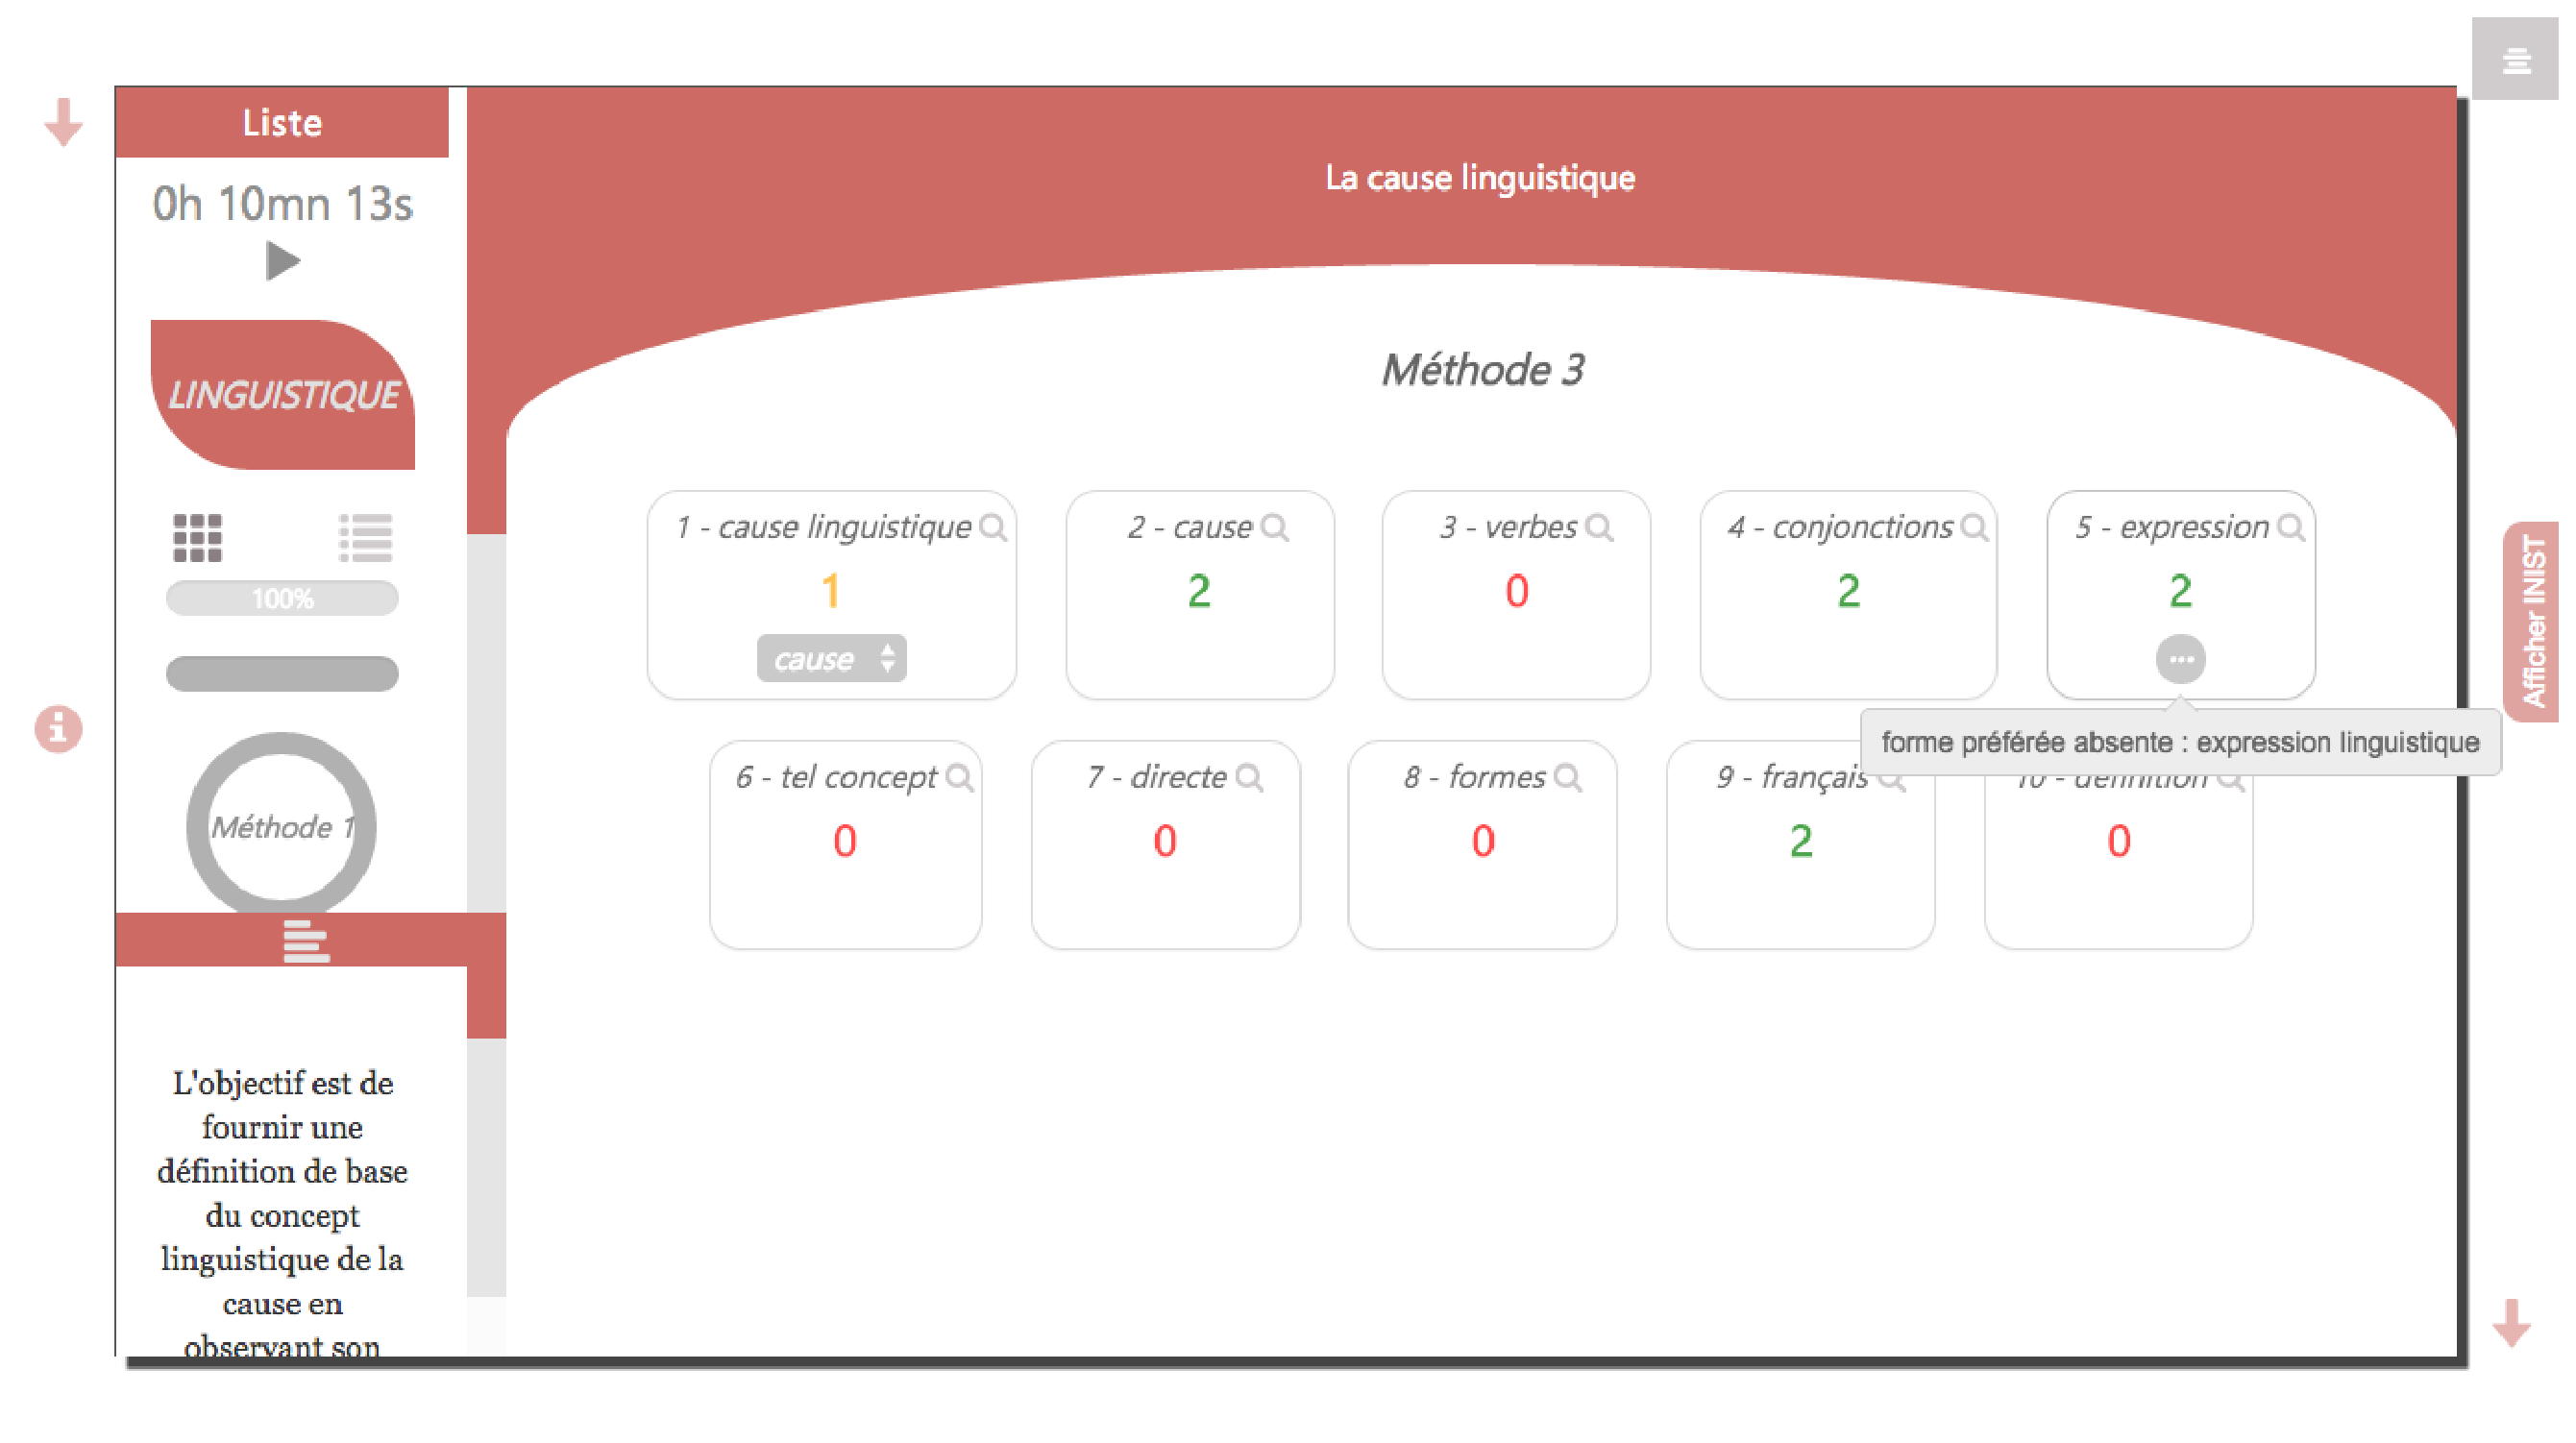
\includegraphics[width=\linewidth]{include/idefix.eps}
          \caption{Interface d'évaluation manuelle de l'Inist
                   \label{fig:idefix}}
        \end{figure}

      \subsubsection{Évaluation du silence}
      \label{subsubsec:main-automatic_evaluation_of_keyphrase_annotation-methodology-evaluation_protocol-silence}
        Pour évaluer le silence, l'évaluateur doit attribuer à chaque terme-clé
        de référence un score indiquant le degré d'importance de l'information
        qu'il véhicule et qui n'est pas capturée par les termes-clés fournis par
        une méthode d'indexation par termes-clés. Sur une échelle de 0 à 2, ce
        score permet d'indiquer s'il n'y pas de perte d'information (0), si
        l'information perdue est capitale (2) ou si elle est secondaire (1).
        Lorsqu'un terme-clé de référence obtient un score de 0, cela signifie
        soit qu'il fait partie des termes-clés fournis par la méthode
        d'indexation par termes-clés, soit que l'indexeur juge qu'il ne devrait
        pas être un terme-clé de référence, c'est-à-dire une erreur parmi les
        termes-clés de référence.

        Une perte d'information est jugée secondaire (score de 1) dans deux
        cas de figure~:
        \begin{itemize}
          \item{terme-clé de référence secondaire~: le terme-clé de référence
                n'apporte pas l'information la plus importante~;}
          \item{terme-clé de référence générique~: le terme-clé de référence
                n'est pas suffisamment spécifique au contenu du document, il a
                un usage classificatoire.}
        \end{itemize}
        Afin de minimiser les pertes d'informations dues à des termes-clés de
        référence qui ne sont pas présents dans le document, les évaluateurs
        leur attribuent un score de 1.

    \subsection{Évaluation manuelle des méthodes proposées}
    \label{subsec:main-domain_specific_keyphrase_annotation-manual_evaluation-analysis}
      Dans cette section, nous analysons l'évaluation manuelle de TopicRank,
      TopicCoRank, d'une méthode de référence non supervisée, \textsc{Tf-Idf},
      et d'une méthode de référence supervisée, \textsc{Kea}\footnote{La raison
      pour laquelle les évaluations
      manuelles sont réalisées sur \textsc{Kea} et non pas \textsc{Kea++} est
      temporelle. L'évaluation manuelle étant coûteuse, nous n'avons pas pu
      la réitérer avec \textsc{Kea++}.}. L'évaluation est
      et d'une méthode de référence, \textsc{Tf-Idf}. L'évaluation est
      effectuée par un indexeur professionnel, sur la collection de linguistique
      Termith.

      Dans un premier temps, nous analysons l'évaluation manuelle de TopicRank
      et la comparons à celle de \textsc{Tf-Idf}, puis, dans un second temps,
      nous analysons l'évaluation manuelle de TopicCoRank et la comparons à
      celle de \textsc{Kea}. Tous les termes-clés sont obtenus à partir des
      documents prétraités, comme nous l'avons présenté dans la
      section~\ref{sec:main-data_description-preprocessing}
      (page~\pageref{sec:main-data_description-preprocessing}). Les candidats
      sont sélectionnés à l'aide du patron grammatical \texttt{/(N|A)+/}.

      \subsubsection{Évaluation de TopicRank}
      \label{subsubsec:main-domain_specific_keyphrase_annotation-manual_evaluation-analysis-topicrank}
        Le
        tableau~\ref{tab:main-automatic_evaluation_of_keyphrase_annotation-results-topicrank-pertinence_score_ratio}
        montre les scores de pertinence moyens de TopicRank et \textsc{Tf-Idf}. Pour le score
        de 1, qui indique qu'un terme-clé est un forme variante, nous
        distinguons le cas où la variante est redondante du cas où elle ne l'est
        pas. Nous observons que TopicRank est meilleur que
        \textsc{Tf-Idf}. TopicRank fournit plus de termes-clés pertinents que
        \textsc{Tf-Idf}, mais fait aussi plus d'erreurs. Les termes-clés ayant
        un score de 1 donnent un explication intéressante à cette
        contradiction~: \textsc{Tf-Idf} à une forte tendance à extraire des
        termes-clés redondants, c'est-à-dire des termes-clés variantes de
        termes-clés déjà extraits, alors que TopicRank remplit son
        objectif de ne pas extraire de termes-clés redondants, avec seulement
        0,9~\% de redondance.
        \begin{table}[h!]
          \centering
          \begin{tabular}{l|c|c|c|c}
            \toprule
            \multirow{2}{*}{\textbf{Méthode}} & \multirow{2}{*}{\textbf{0}} & \multicolumn{2}{c|}{\textbf{1}} & \multirow{2}{*}{\textbf{2}}\\
            \cline{3-4}
            & & \multicolumn{1}{p{.175\linewidth}|}{\centering{}redondant} & \multicolumn{1}{p{.175\linewidth}|}{\centering{}non redondant} &\\
            \hline
            \textsc{Tf-Idf} & \textbf{53,8~\%} & 6,8~\% & 4,2~\% & 35,3~\%\\
            TopicRank & 56,3~\% & \textbf{0,9~\%} & \textbf{5,7~\%} & \textbf{37,1~\%}\\
            \bottomrule
          \end{tabular}
          \caption{Taux de termes-clés avec un score de 0, de 1 ou de 2 pour
                   l'évaluation de la pertinence de \textsc{Tf-Idf} et de
                   TopicRank
                   \label{tab:main-automatic_evaluation_of_keyphrase_annotation-results-topicrank-pertinence_score_ratio}}
        \end{table}

        Les résultats présentés dans le
        tableau~\ref{tab:main-automatic_evaluation_of_keyphrase_annotation-results-topicrank-pertinence_score_ratio}
        sont contraires à ceux de l'évaluation automatique, puisque c'est ici
        TopicRank qui est meilleur que \textsc{Tf-Idf} sur les documents de
        linguistique. Afin de mieux observer la différence entre l'évaluation
        manuelle et l'évaluation automatique, nous calculons la précision (P),
        le rappel (R) et la f1-mesure (F) résultantes de l'évaluation
        manuelle et les comparons aux résultats automatiques que nous avons
        montré dans le tableau~\ref{tab:resultats_inist}
        (page~\pageref{tab:resultats_inist}). Pour calculer ces performances,
        les termes-clés ayant un score de 2 sont considérés corrects, de même
        que ceux ayant un score de 1 non redondants. Les résultats de
        l'évaluation manuelle comparés à ceux de l'évaluation automatique sont
        présentés dans le
        tableau~\ref{tab:main-automatic_evaluation_of_keyphrase_annotation-results-topicrank-prf}.
        
        La difficulté d'évaluer automatiquement la tâche d'indexation par
        termes-clés se confirme. Avec l'évaluation manuelle, les conclusions ne
        sont pas les mêmes, puisque de manière automatique TopicRank est moins
        performant que \textsc{Tf-Idf} alors qu'il est plus performant selon
        l'évaluation manuelle. Nous observons aussi un écart conséquent entre
        les performances évaluées manuellement et celles évaluées
        automatiquement. Le gain d'environ 20 points atteste le pessimisme de
        l'évaluation automatique.
        \begin{table}[h!]
          \centering
          \begin{tabular}{l|c@{~~~~~~}cc|c@{~~~~~~~~}cc}
            \toprule
            \multirow{2}{*}{\textbf{Méthode}} & \multicolumn{3}{c|}{\textbf{Évaluation manuelle}} & \multicolumn{3}{c}{\textbf{Évaluation automatique}}\\
            \cline{2-7}
            & P & R & F & P & R & F\\
            \hline
            \textsc{Tf-Idf} & 39,5 & 29,7 & 33,5 & \textbf{13,0} & \textbf{15,4} & \textbf{13,9}\\
            TopicRank & \textbf{42,8} & \textbf{32,2} & \textbf{36,2} & 11,2 & 13,1 & 11,9\\
            \bottomrule
          \end{tabular}
          \caption[
            Performances de \textsc{Tf-Idf} et de TopicRank en termes de
            précision, de rappel et de f1-mesure
          ]{
            Performances de \textsc{Tf-Idf} et de TopicRank en termes de
            précision (P), de rappel (R) et de f1-mesure (F)
            \label{tab:main-automatic_evaluation_of_keyphrase_annotation-results-topicrank-prf}}
        \end{table}
      
        ~\\Enfin, le
        tableau~\ref{tab:main-automatic_evaluation_of_keyphrase_annotation-results-topicrank-silence_score_ratio}
        montre les scores de silence attribués en moyenne par méthode. D'après
        la description donnée pour chacun des scores, la méthode qui capture le
        plus d'information est celle qui maximise le nombre de termes-clés de
        référence ayant un score de silence 0 et qui minimise ceux ayant un
        score de 1 et de 2. Nous observons donc que TopicRank couvre mieux le
        contenu principal des documents que \textsc{Tf-Idf}. Parce que TopicRank
        groupe les termes-clés candidats en sujets et n'extrait qu'un seul
        terme-clé par sujet, il y a moins de redondance parmi les termes-clés
        qu'il extrait (cf
        tableau~\ref{tab:main-automatic_evaluation_of_keyphrase_annotation-results-topicrank-pertinence_score_ratio})
        et le nombre de sujets couverts est donc meilleur.
        \begin{table}[h!]
          \centering
          \begin{tabular}{l|c|c|c}
            \toprule
            \textbf{Méthode} & \textbf{0} & \textbf{1} & \textbf{2}\\
            \hline
            \textsc{Tf-Idf} & 31,4~\% & 48,5~\% & 20,1~\%\\
            TopicRank & \textbf{35,0~\%} & \textbf{48,3~\%} & \textbf{16,8~\%}\\
            \bottomrule
          \end{tabular}
          \caption{Taux de termes-clés de référence avec un score de 0, de 1 ou
                   de 2 pour l'évaluation du silence de \textsc{Tf-Idf} et de
                   TopicRank
                   \label{tab:main-automatic_evaluation_of_keyphrase_annotation-results-topicrank-silence_score_ratio}}
        \end{table}

      \subsubsection{Évaluation de TopicCoRank}
      \label{subsubsec:main-domain_specific_keyphrase_annotation-manual_evaluation-analysis-topiccorank}
        Les résultats que nous montrons dans cette section sont obtenus avec
        seulement 25~\% de l'ensemble de test de la collection linguistique
        Termith\footnote{En raison de cette incomplétude de l'évaluation
        manuelle, nous ne comparons pas l'évaluation manuelle à l'évaluation
        automatique comme nous l'avons fait pour TopicRank et \textsc{Tf-Idf}.}.
        Les différentes revues qui composent la collection sont
        réparties de manière homogène dans ces 25~\%.

        Le
        tableau~\ref{tab:main-domain_specific_keyphrase_annotation-manual_evaluation-analysis-topiccorank-pertinence_score_ratio}
        montre les scores de pertinence moyens de TopicCoRank et \textsc{Kea}.
        Nous observons que TopicCoRank est meilleur que
        \textsc{Kea}. TopicCoRank fournit plus de termes-clés pertinents que
        \textsc{Kea}, mais fait aussi plus d'erreurs. À l'instar de TopicRank,
        TopicCoRank est moins redondant que la méthode de référence. Il est tout
        de même plus redondant que TopicRank. Cela est du au fait qu'il peut assigner un terme-clé et
        extraire une variante pouvant être jugée importante, car plus
        spécifique, ou redondante.
        \begin{table}[h!]
          \centering
          \begin{tabular}{l|c|c|c|c}
            \toprule
            \multirow{2}{*}{\textbf{Méthode}} & \multirow{2}{*}{\textbf{0}} & \multicolumn{2}{c|}{\textbf{1}} & \multirow{2}{*}{\textbf{2}}\\
            \cline{3-4}
            & & \multicolumn{1}{p{.175\linewidth}|}{\centering{}redondant} & \multicolumn{1}{p{.175\linewidth}|}{\centering{}non redondant} &\\
            \hline
            \textsc{Kea} & \textbf{45,2~\%} & 10,2~\% & \textbf{8,0~\%} & 36,6~\%\\
            TopicCoRank & 49,8~\% & \textbf{4,4~\%} & 6,2~\% & \textbf{39,6~\%}\\
            \bottomrule
          \end{tabular}
          \caption{Taux de termes-clés avec un score de 0, de 1 ou de 2 pour
                   l'évaluation de la pertinence de \textsc{Kea} et de
                   TopicCoRank
                   \label{tab:main-domain_specific_keyphrase_annotation-manual_evaluation-analysis-topiccorank-pertinence_score_ratio}}
        \end{table}

        Comparé à TopicRank, TopicCoRank est effectivement plus performant. Il
        trouve plus de termes-clés corrects et fait moins d'erreurs. Cependant,
        comme nous
        l'avons dit ci-dessus, il est plus redondant. Comparée à
        \textsc{Tf-Idf} et \textsc{Kea}, cette redondance est tout de même plus
        faible.

%        \TODO{\dots}
%        \begin{table}[h!]
%          \centering
%          \begin{tabular}{l|c@{~~~~~~}cc|c@{~~~~~~~~}cc}
%            \toprule
%            \multirow{2}{*}{\textbf{Méthode}} & \multicolumn{3}{c|}{\textbf{Évaluation manuelle}} & \multicolumn{3}{c}{\textbf{Évaluation automatique}}\\
%            \cline{2-7}
%            & P & R & F & P & R & F\\
%            \hline
%            \textsc{Kea} & 44,6 & 32,5 & 37,1 & 13,8 & 16,3 & 14,7\\
%            TopicCoRank & \textbf{45,8} & \textbf{34.1} & \textbf{39.6} & \textbf{19,0} & \textbf{22,0} & \textbf{20,1}\\
%            \bottomrule
%          \end{tabular}
%          \caption[
%            Performances de \textsc{Kea} et de TopicCoRank en termes de
%            précision, de rappel et de f-mesure
%          ]{
%            Performances de \textsc{Kea} et de TopicCoRank en termes de
%            précision (P), de rappel (R) et de f-mesure (F)
%            \label{tab:main-domain_specific_keyphrase_annotation-manual_evaluation-analysis-topiccorank-prf}}
%        \end{table}
      
        ~\\Enfin, le
        tableau~\ref{tab:main-domain_specific_keyphrase_annotation-manual_evaluation-analysis-topiccorank-silence_score_ratio}
        montre les scores de silence attribués en moyenne par méthode. Les
        conclusions qu'ils induisent ne sont pas en faveur de
        TopicCoRank. En effet, même s'il ne capture pas autant de termes-clés
        que TopicCoRank, \textsc{Kea} capture ceux qui sont sémantiquement les
        plus indispensables. Bien que les deux méthodes sont supervisées,
        \textsc{Kea} est la seule des deux à apprendre à détecter les
        termes-clés à partir des traits des termes-clés du domaine. Si
        l'ordonnancement conjoint à base de graphe est plus efficace pour
        identifier les termes-clés, l'apprentissage permet une meilleure
        précision quant à l'identification de ceux les plus indispensables.
        \begin{table}[h!]
          \centering
          \begin{tabular}{l|c|c|c}
            \toprule
            \textbf{Méthode} & \textbf{0} & \textbf{1} & \textbf{2}\\
            \hline
            \textsc{Kea} & \textbf{37,3~\%} & 46,0~\% & \textbf{16,7}~\%\\
            TopicCoRank & 35,9~\% & \textbf{45,3~\%} & 18,8~\%\\
            \bottomrule
          \end{tabular}
          \caption{Taux de termes-clés de référence avec un score de 0, de 1 ou
                   de 2 pour l'évaluation du silence de \textsc{Kea} et de
                   TopicCoRank
                   \label{tab:main-domain_specific_keyphrase_annotation-manual_evaluation-analysis-topiccorank-silence_score_ratio}}
        \end{table}

    \subsection{Bilan}
    \label{subsec:main-domain_specific_keyphrase_annotation-manual_evaluation-conclusion}
      Nous avons réalisé une campagne d'évaluation manuelle de nos travaux en
      domaine de spécialité, avec la collection de linguistique Termith. Pour
      cette campagne, nous avons proposé un protocole d'évaluation et des
      métriques permettant de capturer deux aspects de l'indexation par
      termes-clés~: la pertinence des termes-clés extraits/assignés et leur
      silence, c'est-à-dire la quantité d'information importante qu'ils ne
      capturent pas. Contrairement au premier aspect, qui est similaire à ce
      qu'évalue un système automatique, le dernier aspect permet d'évaluer les
      termes-clés d'un point de vu sémantique, jamais considéré auparavant.

      Les résultats montrent que, contrairement à ce que montrait l'évaluation
      automatique, TopicRank effectue une indexation par termes-clés de
      meilleure qualité que celle de \textsc{Tf-Idf}. TopicRank extrait peu de
      termes-clés redondants et couvre mieux le document, en partie grâce à son
      groupement des termes-clés candidats en sujets. Entre TopicCoRank,
      TopicRank, \textsc{Tf-Idf} et \textsc{Kea}, c'est TopicCoRank qui trouve
      le plus de termes-clés corrects. L'évaluation du silence montre tout de
      même que c'est \textsc{Kea} qui identifie ceux jugés les plus
      indispensables par les indexeurs professionnels. Les deux aspects
      (pertinence et silence) de l'évaluation manuelle et leurs conclusions
      paradoxales soulèvent une nouvelle perspective pour l'évaluation
      automatique. En effet, il serait intéressant d'ordonner par importance les
      termes-clés de référence et d'en tenir compte pour identifier les méthodes
      qui capturent les termes-clés les plus indispensables.

  %-----------------------------------------------------------------------------

  \section{Conclusion}
  \label{sec:main-domain_specific_keyphrase_annotation-conclusion}
    Nous nous sommes intéressé à l'indexation automatique par termes-clés en
    domaines de spécialité. Nous avons tout d'abord présenté l'indexation
    manuelle réalisée par des indexeurs professionnels dans ce contexte, nous
    avons ensuite proposé une nouvelle méthode automatique se rapprochant le
    plus possible de cette indexation, puis nous avons présenté les premiers
    résultats d'une campagne d'évaluation manuelle que nous avons réalisé avec
    des indexeurs professionnels.

    Contrairement aux méthodes d'indexation automatique, l'indexation manuelle
    n'est pas divisée entre extraction et assignement. L'indexation manuelle en
    domaines de spécialité préfère l'assignement, car cela permet une
    indexation homogène des documents d'un même domaine et une conformité
    vis-à-vis du vocabulaire spécialisé du domaine. Elle a aussi besoin de
    l'extraction, afin de fournir des termes-clés très spécifiques au document,
    ainsi que pour y identifier d'éventuels nouveaux concepts.

    Pour remédier à la fracture entre extraction et assignement en indexation
    automatique par termes-clés, nous proposons TopicCoRank. Conçu sur la base
    de TopicRank, TopicCoRank utilise les données d'entraînement pour
    représenter le domaine avec un graphe unifié à celui des sujets. Cette
    unification permet d'améliorer l'ordonnancement des sujets, en tenant compte
    de leurs relations avec le domaine, et d'assigner des termes-clés, en
    puisant dans le domaine. À notre connaissance, TopicCoRank est la seule
    méthode qui réalise conjointement extraction et assignement.

    Pour valider les deux méthodes TopicRank et TopicCoRank, nous avons réalisé
    une campagne d'évaluation manuelle en domaine de spécialité. Le protocole
    d'évaluation que nous avons proposé permet d'évaluer chaque méthode selon le
    degré de pertinence des termes-clés qu'elle propose et selon le degré
    d'information qui lui échappe. Les résultats de l'évaluation manuelle de
    TopicRank son plus encourageant que ceux de l'évaluation automatique. Ils
    montrent que TopicRank est en réalité plus performant que \textsc{Tf-Idf},
    en partie parce qu'il couvre mieux les sujets du document grâce à son
    groupement en sujets des termes-clés candidats.
    Ils montrent aussi que TopicCoRank est la méthode la plus performante
    comparée à TopicRank, \textsc{Tf-Idf} et \textsc{Kea}. Cependant, c'est
    \textsc{Kea} qui trouve les termes-clés les plus indispensables.
    Au delà de cela, cette
    campagne a montré les limites de l'évaluation automatique, qui suit un
    paradigme trop strict pour la tâche d'indexation par termes-clés. Parce que
    l'évaluation manuelle est trop coûteuse pour être systématiquement mise en
    \oe{}uvre, il est donc important de s'intéresser de plus près aux méthodes
    d'évaluation automatique. Les ressources de notre campagne, annotées étape
    par étape, seront donc
    rendues disponibles gratuitement à toute la communauté scientifique. Cette
    disponibilité permettra d'évaluer de nouvelles méthodes d'évaluation, en
    vérifiant leur corrélation avec l'évaluation manuelle des indexeurs
    professionnels.

